% Plantilla básica para ejemplar formal oficial de tesis de la Escuela Internacional de Doctorado (EIDUM) 
% de la Universidad de Murcia, España. (ejemplar formal)
% Antonio Maurandi López, 8 de marzo de 2023
%
% Notas: 
% - el dir "estilos" contiene un fichero variables.tex donde poner titulo, autor, etc... y otros de librerías etc...
% - en el dir "capitulos" van los capítulos a inc con un input
% - otro dir de "capitulos/tablas" para editarlas tranquilamente e inc con un input tb.
% - en el directorio "pics" pongo las imágenes
% - la biblio no es APA, pq no me gusta, tampoco es obligatorio q así lo sea.
% -
% ---------------------------------------------------------

\documentclass[a4paper,12pt,oneside]{book}
% phd-estilo-basico.tex
% aml! 2015-09-08. amaurandi@um.es
% ------------------------------------------------

%\documentclass[a4paper,12pt]{book}
%\documentclass[11pt]{book}
%\usepackage[paperwidth=17cm, paperheight=22.5cm, bottom=2.5cm, right=2.5cm]{geometry}
\usepackage{amssymb,amsmath} %paquete para símbolo matemáticos
%\usepackage{apacite} %para usar APA cite en bibligrafia tb modificar
\usepackage[spanish, es-tabla, es-nodecimaldot]{babel}  % ponemos tabla en vez de cuadro, sep decimal el punto (Us- notation)

%\usepackage{ucs}
\usepackage[utf8]{inputenc} %Paquete para escribir acentos y otros símbolos directamente

\usepackage{pdflscape}
\usepackage{multirow, booktabs, caption,longtable}
\usepackage{tikz}

\DeclareCaptionLabelSeparator*{spaced}{\\[2ex]}
\captionsetup[table]{textfont=it,format=plain,justification=justified,
  singlelinecheck=false,labelsep=spaced,skip=0pt}
\captionsetup[figure]{labelsep=period,labelfont=it,justification=justified,
  singlelinecheck=false,font=doublespacing}

\usepackage[figuresleft]{rotating}
\usepackage{enumerate}
\usepackage{graphicx}
\usepackage[nottoc]{tocbibind}

% Numeracion de los teoremas y demas con theorem
\usepackage{theorem}
\newtheorem{theorem}{Teorema}[chapter]
\newtheorem{proposition}[theorem]{Proposición}
\newtheorem{corollary}[theorem]{Corolario}
\newtheorem{lemma}[theorem]{Lema}
\newtheorem{definition}[theorem]{Definición}
\newtheorem{remark}[theorem]{Observación}
\newtheorem{example}[theorem]{Ejemplo}
\newtheorem{exercise}[theorem]{Ejercicio}	
%\def\theequation{\thesection.\arabic{equation}}
%\def\thetheo{\thesection.\arabic{theo}}
\newenvironment{proof}{\ignorespaces\par\noindent\textit{Demostración.}\quad}{\hfill$\Box$\par}
\newenvironment{resolve}{\ignorespaces\par\noindent\textit{Resolución.}\quad}{\hfill$\Box$\par}
\newenvironment{notation}{\ignorespaces\par\noindent\textit{Notación.}}{\hfill\par}

%\usepackage{showframe}
\usepackage{enumitem}
\usepackage{centernot}
\usepackage{dsfont}
\newcommand{\card}{\operatorname{Card}}
\newcommand{\floor}[1]{\lfloor #1 \rfloor}
\newcommand{\ceil}[1]{\lceil #1 \rceil}
\newcommand{\partfrac}[1]{\langle #1 \rangle}

% Indentacion
%\usepackage{indentfirst}
\setlength{\parindent}{0cm}
\setlength{\parskip}{3mm}


%\usepackage[pdftex,
%            pdfauthor={Your Name},
%            pdftitle={The Title},
%            pdfsubject={The Subject},
%            pdfkeywords={Some Keywords},
%            pdfproducer={Latex with hyperref, or other system},
%            pdfcreator={pdflatex, or other tool}]{hyperref}

\usepackage[
			%paperwidth=17cm,     % como hago para que trome A4 (sin meterle los cms)???
			%paperheight=23.5cm,
			a4paper, 
			inner=2cm, 
			outer=2cm, 
			top=2.5cm, 
			bottom=2cm, 
			%bindingoffset=1cm
			]{geometry}

\setlength{\captionmargin}{20pt}

%\usepackage[table, xcdraw]{xcolor}

% bloques verbarin coloreados segun estilo Rstudio para código R
% ------------------------------------------------
\usepackage{color}
\usepackage{fancyvrb}
\newcommand{\VerbBar}{|}
\newcommand{\VERB}{\Verb[commandchars=\\\{\}]}
\DefineVerbatimEnvironment{Highlighting}{Verbatim}{commandchars=\\\{\}}
% Add ',fontsize=\small' for more characters per line
\usepackage{framed}
\definecolor{shadecolor}{RGB}{248,248,248}
\newenvironment{Shaded}{\begin{snugshade}}{\end{snugshade}}
\newcommand{\KeywordTok}[1]{\textcolor[rgb]{0.13,0.29,0.53}{\textbf{{#1}}}}
\newcommand{\DataTypeTok}[1]{\textcolor[rgb]{0.13,0.29,0.53}{{#1}}}
\newcommand{\DecValTok}[1]{\textcolor[rgb]{0.00,0.00,0.81}{{#1}}}
\newcommand{\BaseNTok}[1]{\textcolor[rgb]{0.00,0.00,0.81}{{#1}}}
\newcommand{\FloatTok}[1]{\textcolor[rgb]{0.00,0.00,0.81}{{#1}}}
\newcommand{\CharTok}[1]{\textcolor[rgb]{0.31,0.60,0.02}{{#1}}}
\newcommand{\StringTok}[1]{\textcolor[rgb]{0.31,0.60,0.02}{{#1}}}
\newcommand{\CommentTok}[1]{\textcolor[rgb]{0.56,0.35,0.01}{\textit{{#1}}}}
\newcommand{\OtherTok}[1]{\textcolor[rgb]{0.56,0.35,0.01}{{#1}}}
\newcommand{\AlertTok}[1]{\textcolor[rgb]{0.94,0.16,0.16}{{#1}}}
\newcommand{\FunctionTok}[1]{\textcolor[rgb]{0.00,0.00,0.00}{{#1}}}
\newcommand{\RegionMarkerTok}[1]{{#1}}
\newcommand{\ErrorTok}[1]{\textbf{{#1}}}
\newcommand{\NormalTok}[1]{{#1}}
% ------------------------------------------------

\usepackage{pdfpages} % insertar pdf en los anexos
%\usepackage{cite} % para contraer referencias

\usepackage{fancyhdr}
\pagestyle{fancy}

\usepackage{placeins}  % para usar \FloatBarrier
%\usepackage{minitoc}
\usepackage{float}
\usepackage{url}

\usepackage{lipsum}
%\usepackage{setspace}

\usepackage[backend=biber]{biblatex}
\usepackage{hyperref}
%\usepackage{apacite} %para usar APA cite en bibligrafia tb modificar \bibliographystyle{apacite} en su ssitio 
%\DefineBibliographyStrings{spanish}{ andothers = {et\addabbrvspace al\adddot}, and = {y}, }
%\renewcommand{\BOthers}[1]{et al.\hbox{}}
%\addto\captionsspanish{
%   \renewcommand{\BOthers}[1]{et al.\hbox{}}
%}

\usepackage[normalem]{ulem} %para tachar frases

%aml para solventar el tema de las citas intex.. 20220405
%\usepackage[sort&compress,square,comma,authoryear]{natbib}


% makes color citations
%\usepackage[colorlinks=true,urlcolor=blue,citecolor=red,linkcolor=red,bookmarks=true]{hyperref}
\setlength{\jot}{5pt}
 
\input{./estilos/estilo-capitulos.tex}
\newcommand{\variableTituloTesis}{El teorema de equidistribución de Weyl}
\newcommand{\variableTesinando}{Domingo Antonio Manzanares Sánchez}
\newcommand{\variableAnho}{2025-2026}

\newcommand{\variableDireccionUno}{Prof. D. Gustavo Adolfo Garrigós Aniorte}
\newcommand{\variableDireccionDos}{}
\newcommand{\variableDireccionTres}{}






\addbibresource{./bibliografia.bib}
\begin{document}
%-------------------------------------------------------------------
%	PORTADA
%-------------------------------------------------------------------
\pagestyle{empty}
% portada.tex


\vspace{28.5mm}
%Figura
\begin{figure}[h]
    \begin{center}
        
\includegraphics[width=72mm]{pics/institucional/escudo-um-bn.png}
    \end{center}
\end{figure}


\begin{center}



%\vspace{7.5mm}
\textsc{\Large UNIVERSIDAD DE MURCIA}\\[4em]

%\vspace{28mm}
\textsc{\Large FACULTAD DE MATEMÁTICAS}\\[4em]


\vspace{20mm}
\textsc{\Large \variableTituloTesis} 

%\textsc{\Large Bla Bla Bla Bla  Bla Bla  Bla Bla  Bla Bla Bla Bla  Bla Bla  Bla Bla  
        %\\y bla bla bla bla  bla bla  bla bla  bla bla bla bla  bla bla  bla bla  
    %} 



\vspace{60.5mm}
\textsc{\Large \variableTesinando}\\[1em]
\textsc{\Large \variableAnho}\\[1em]

%\large Directoras: \\ Prof. Dra. Dña. Laura del Río Alonso\\ Prof. Dr. D. Fulanito de tal y cual\\ Prof. Dr. D. Menganito de tal y cual


\end{center}

\vspace*{\fill}


%\end{titlepage}





\newpage 
\ % pagina ne blanco
\newpage
% CONTRAPORTADA con nombres de directoras
% portada.tex

\FloatBarrier
\vspace{28.5mm}
%Figura
\begin{figure}[H]
    \begin{center}
        
\includegraphics[width=82mm]{pics/institucional/SelloUMU-positivo.png}
    \end{center}
\end{figure}


\begin{center}



%\vspace{7.5mm}
\textsc{\Large UNIVERSIDAD DE MURCIA}\\[4em]

%\vspace{28mm}
\textsc{\Large FACULTAD DE MATEMÁTICAS}\\[4em]


\vspace{20mm}
\textsc{\Large \variableTituloTesis} 



\vspace{20mm}
\textsc{\Large \variableTesinando}\\[1em]
\textsc{\Large \variableAnho}\\[1.5 em]
\textsc{\large Dirección: \\ \variableDireccionUno} 


\end{center}

\vspace*{\fill}


%\end{titlepage}





%\newpage

%-------------------------------------------------------------------
%	Frase Culterana
%-------------------------------------------------------------------
%\pagestyle{empty}
\frontmatter
\chapter*{}
% fraseculterana.tex

\begin{flushright}
    \textit{Lasciate ogni speranza, voi ch'entrate.\\
     Dante Alighieri}
\end{flushright}




%-------------------------------------------------------------------
%	DEDICATORIA
%-------------------------------------------------------------------
%\pagestyle{empty}
\frontmatter
\chapter*{}
%dedicatoria.tex
\begin{flushright}
    \begin{minipage}{0.35\textwidth}
    \small
    A mis padres, a mi hermana, a mi tutor, y a todas las personas que me han acompañado ---familiares y amigos--- durante la carrera.
    \end{minipage}
\end{flushright}

%-------------------------------------------------------------------
%	AGRADECIMIENTOS
%-------------------------------------------------------------------
\chapter*{Agradecimientos}
%\markboth{AGRADECIMIENTOS23}{AGRADECIMIENTOS} % encabezado 
\input{./elementos/resto/Z-agradecimientos.tex}

%-------------------------------------------------------------------
%	PREFACIO
%-------------------------------------------------------------------
\chapter*{Prefacio}


% Este trabajo de investigación es origen de varias publicaciones científicas, las dos primeras son requisito del Programa de Doctorado en Educación de la Universidad de Murcia,  al que pertenece, la tercera es adicional.


% \textbf{Congreso Internacional}

% Arteaga Marin, M. I., Olivares Carrillo, P. y Maurandi López, A. (2022). Metodologías activas en el proceso educativo: recomendaciones para una
% implementación eficaz en educación básica y bachillerato para la enseñanza
% STEM. \textit{3rd edition of Porto International Conference on Research in Education},
% \url{https://porto-icre2022.eventqualia.net/en/2022/home/}.

% \textbf{Artículos Indexados}

% \textcolor{red}{Latindex}. Arteaga-Marín, M. I. ., Sánchez-Rodríguez, A. ., Olivares-Carrillo,P., y Maurandi-López, A. (2022). Revisión sistemática y propuesta para la implementación de metodologías activas en la educación STEM. \textit{EDUCATECONCIENCIA, 30}(36), 35-76, \url{https://tecnocientifica.com.mx/educateconciencia/index.php/revistaeducate/article/view/533}. ISSN: 2683-2836

% \textcolor{red}{Scopus Q1}. Ibáñez-López, F. J.; Arteaga-Marín, M.; Olivares-Carrillo, P.; Sánchez-Rodríguez, A.; Maurandi-López, A. (2022). Diseño y validación de un cuestionario sobre uso de herramientas tecnológicas en innovación de asignaturas STEM. \textit{Campus Virtuales, 11}(2), 179-195, \url{https://doi.org/10.54988/cv.2022.2.1081. ISSN: 2255-1514}

% \begin{center}
%     \includegraphics[width=0.8\textwidth]{pics/publicaciones.png}
% \end{center}

%En este trabajo emplearemos las siguientes convenciones: 

%\begin{itemize}
%\item 
%Se empleará la tipografía \textit{cursiva} para palabras en otro idioma distinto del castellano y para resaltar nombres como, por ejemplo, los nombres de variables.
%\item 
%Emplearemos la tipografía \texttt{código} para sentencias de código,  nombres de funciones y librerías de \texttt{R}.
%\item 
%Emplearemos el punto como separador decimal, por ejemplo: \texttt{1/2=0.5}, y un espacio simple como separador de millares, por ejemplo: \texttt{123\;345} tal como recomienda la Academia de la Lengua Española en la Ortografía del 2010, página 666 \cite{espanola2010ortografia}. 
%\item 
%Cuando informemos sobre una media, la acompañaremos entre paréntesis de la desviación típica, por ejemplo: \texttt{8.81(1.21)}. 
%\item 
%Si informamos de un porcentaje, entre paréntesis, incluimos la frecuencia absoluta, por ejemplo: \texttt{50.25\%(123)}, o viceversa: \texttt{123(50.25\%)}. 
%\item 
%En las tablas de descriptivos, empleamos la abreviatura \texttt{SD} para \emph{desviación estandar} (del inglés \emph{Standard  Deviation}).
%\item 
%En el texto empleamos la abreviatura \texttt{EPV} para \emph{Enfermedades Prevenibles por Vacunas}.
%\end{itemize}



%-------------------------------------------------------------------
%	RESUMEN y SUMMARY para la versión oficial
%-------------------------------------------------------------------
\chapter*{Resumen y Summary}
\input{./elementos/resto/Z-resumenYsummary.tex}

%-------------------------------------------------------------------
%	TABLA DE CONTENIDOS
%-------------------------------------------------------------------
%\setcounter{tocdepth}{1}
%level -1: part, 0: chapter, 1: section, etc.
\renewcommand{\baselinestretch}{0.1}\normalsize
\tableofcontents
\renewcommand{\baselinestretch}{0.3}\normalsize
\listoffigures
\renewcommand{\baselinestretch}{0.3}\normalsize
%\listoftables
\renewcommand{\baselinestretch}{1.2}\normalsize

%-------------------------------------------------------------------
%	TESIS
%-------------------------------------------------------------------
\mainmatter %empieza la numeración de las páginas
\pagestyle{headings}

\def\tablename{Tabla}% para que denomine tabla a las tablas y no "cuadro"
%\doublespacing
\onehalfspace
%\singlespace
%\spacing{1.5}	
%\setlength{\parskip}{3mm}% separación entre párrafo
%\setlength{\parindent}{1cm}%identación primera linea de párrafo


\chapter{Equidistribución módulo 1}
Durante años, el estudio de las sucesiones ha sido fundamental en la teoría de 
números y en el análisis. Una de las sucesiones más relevantes es la sucesión formada
por las partes fraccionarias de los múltiplos de un número real $\alpha$,
\[
  \partfrac{\alpha}, \, \partfrac{2\alpha}, \, \partfrac{3\alpha}, \, \ldots, \, \partfrac{n\alpha}, \, \ldots
\]
donde $\partfrac{x}$ es la parte fraccionaria de $x$. 

El comportamiento de esta sucesión depende de $\alpha$. Si es racional, la 
sucesión es periódica y toma un número finito de valores. Sin embargo, cuando 
$\alpha$ es irracional, la sucesión deja de ser periódica y no se repite. 
En este caso, surge la pregunta de cómo se distribuyen los valores. 

En el siglo XIX, Kronecker demostró que si $\alpha$ es irracional, 
entonces la sucesión es densa en el intervalo $[0,1)$. Más tarde, entre 1909 y
1910, Bohl, Sierpiński y Weyl demostraron de manera independiente que esta 
sucesión no solo es densa, sino que también es equidistribuida. Este último,
Weyl, desarrolló una teoría general para el estudio de la distribución de 
sucesiones en~$[0,1)$.

En este capítulo, exploraremos los conceptos básicos para estudiar este tipo 
de problemas y los usaremos para demostrar el resultado Weyl, la equidistribución
de la sucesión $\partfrac{n\alpha}$ cuando $\alpha$ es un número irracional. 

\section{Números reales módulo 1}

\begin{definition}
    Se define la parte entera de un número $x\in \mathbb{R}$ como 
    \[
        \floor{x} = \max \{k \in \mathbb{Z}: k \leq x\}.
    \]
\end{definition} 

\begin{definition}
    Se define la parte fraccionaria de un número $x\in \mathbb{R}$ como
    \[
        \partfrac{x} = x - \floor{x}.
    \]
    Por definición, se tiene que $\partfrac{x} \in [0,1)$ para todo $x \in \mathbb{R}$.
\end{definition}

Ahora, en $\mathbb{R}$, consideramos la relación de equivalencia dada por $x \sim y$ 
si y solo si $x - y \in \mathbb{Z}$. Es decir, dos números son congruentes
módulo $\mathbb{Z}$ o módulo $1$ si difieren por un número entero. Lo indicamos con
\[
    x \equiv y \mod \mathbb{Z} \qquad \text{ o } \qquad x \equiv y \mod 1
\]

Cada clase de equivalencia tiene un representante único en el intervalo $[0,1)$ que es
justamente la parte fraccionaria $\partfrac{x}$. Podemos pensar en el conjunto cociente 
$\mathbb{R}/\mathbb{Z}$ como el intervalo $[0,1)$ al identificar sus extremos $0$ y $1$.
Este espacio se denota por $\mathbb{T}$, el toro unidimensional o la circunferencia unitaria.

A lo largo del trabajo, utilizaremos $\mathbb{T}$ para referirnos al intervalo $[0,1)$ 
con la identificación de sus extremos. 

\begin{remark}
    Las funciones en $\mathbb{T}$ son funciones $f$ $1$-periódicas en $\mathbb{R}$. Es decir,
    \[
        f(x+1) = f(x) \quad \text{ para todo } x \in \mathbb{R}.
    \]
    Debido a esta periodicidad, tenemos que $f(x) = f(\partfrac{x})$ para todo $x \in \mathbb{R}$,
    por lo que podemos considerar a $f$ como una función definida en $\mathbb{T}$.
\end{remark}

\section{Equidistribución de sucesiones}

\begin{definition}
    Sea $x=(x_n)_{n\geq1}$ una sucesión de números reales. Decimos que $(x_n)$ es
    equidistribuida módulo $1$ si para cada
    intervalo $(a,b) \subset \mathbb{T}$ con $0 < a < b < 1$ se cumple que
    \begin{align}
        \label{def:equidistribucion}
        \lim_{N\to\infty} \frac{A_N((a,b), x)}{N} = b-a
    \end{align}
    donde 
    \[
        A_N((a,b), x) = \card \left\{1\le n\le N : \partfrac{x_n} \in (a,b)\right\}
    \]
\end{definition}

\begin{remark}
    \label{obs:equidistribucion}
    Si consideramos la función característica $\mathbf{1}_{(a,b)}$ en $\mathbb{T}$, entonces la
    condición de equidistribución se puede reescribir como
    \[
        \lim_{N\to\infty} \frac{1}{N} \sum_{n=1}^N \mathbf{1}_{(a,b)}(x_n) =
        \int_0^1 \mathbf{1}_{(a,b)}(x)\ dx = 
        b-a
    \]
\end{remark}

Podemos pensar que, cuando una sucesión es equidistribuida módulo $1$, sus términos se distribuyen
de manera equitativa a lo largo de $\mathbb{T}$. En particular, la proporción de términos que 
pertenecen a un subintervalo es igual a la longitud de dicho intervalo.

La siguiente proposición permite utilizar cualquier tipo de intervalo para
verificar la equidistribución de una sucesión.

\begin{proposition}
    \label{prop:equivalentes}
    Sea $x=(x_n)_{n\geq1}$ una sucesión de números reales.
    Las siguientes afirmaciones son equivalentes:
    \begin{enumerate}
        \item $(x_n)$ es equidistribuida módulo $1$.

        \item La igualdad (\ref{def:equidistribucion}) se cumple
        para todo intervalo $(a,b)$ con $0 \leq a < b \leq 1$.

        \item La igualdad (\ref{def:equidistribucion}) se cumple
        para todo intervalo $[a,b], \,[a,b), \,(a,b]$ con $0 \leq a < b \leq 1$.

        \item La igualdad (\ref{def:equidistribucion}) se cumple
        para todo intervalo $[0,b)$ con $0 \leq b \leq 1$.

        \item La igualdad (\ref{def:equidistribucion}) se cumple
        para todo intervalo $(a,1)$ con $0 \leq a \leq 1$.

        \item La igualdad (\ref{def:equidistribucion}) se cumple
        para todo intervalo $(a,b)$ con $a,b\in D$, donde $D \subseteq \mathbb{T}$ es un conjunto denso.
    \end{enumerate}
\end{proposition}

\begin{proof}
    La demostración es técnica y se incluye en el apéndice \ref{def:equivalentes}.
\end{proof}

\begin{proposition}
    \label{prop:quitar_terminos}
    Sea $x=(x_n)_{n\geq1}$ una sucesión equidistribuida módulo $1$.  Si eliminamos
    un número finito de términos, la sucesión resultante sigue siendo equidistribuida módulo $1$.
\end{proposition}

\begin{proof}
    Sin pérdida de generalidad, supongamos que eliminamos los primeros $M$ términos de la sucesión 
    y sea $y=(y_n)_{n\geq1}$, definimos $y_n = x_{n+M}$ para cada $n \in \mathbb{N}$. 
    
    Sea $(a,b) \subset \mathbb{T}$,    
    \[
        A_N((a,b),y) = \card \left\{M+1 \leq n \leq N+M : \partfrac{x_n} \in (a,b)\right\}
    \]
    por lo que,
    \[
        A_N((a,b),y) = A_{N+M}((a,b),x) - A_M((a,b),x)
    \]

    Como $0 \leq A_M((a,b),x) \leq M$ y la sucesión $(x_n)$ es equidistribuida, 
    \[
        \lim_{N \to \infty} \frac{A_N((a,b),y)}{N} =
        \lim_{N \to \infty}  \left(\frac{N+M}{N} \, \frac{A_{N+M}((a,b),x)}{N+M} - \frac{A_M((a,b),x)}{N} \right) =
        b-a
    \]

    Por lo tanto, la sucesión $(y_n)$ es equidistribuida módulo $1$.
\end{proof}


\begin{proposition}
    \label{prop:secuencia_mas_const}
    Sea $x=(x_n)_{n\geq1}$ una sucesión equidistribuida módulo $1$
    y sea $\alpha \in \mathbb{R}$. Entonces la sucesión $y=(y_n)_{n\geq1}$ dada por
    $
        y_n = x_n + \alpha
    $
    también es equidistribuida módulo $1$.
\end{proposition}

\begin{proof}
    Sea $I=(a,b) \subset \mathbb{T}$ con $0 < a < b < 1$, definimos $J = I - \alpha \mod 1$.
    Para cada $n \in \mathbb{N}$, tenemos que
    \[
        \partfrac{y_n} \in I
        \iff \partfrac{x_n + \alpha} \in I
        \iff \partfrac{x_n} \in J
    \]
    luego
    \[
        A_N(I,y)=A_N(J,x)
    \]

    Como $(x_n)$ es equidistribuida módulo $1$ y la medida es invariante por traslaciones, se tiene
    \[
        \lim_{N\to\infty} \frac{A_N(I,y)}{N} =
        \lim_{N\to\infty} \frac{A_N(J,x)}{N} =
        |J|=|I|
    \]
    demostrando que $(y_n)$ es equidistribuida módulo $1$.
\end{proof}


\begin{example}
    Consideremos una sucesión de racionales $r=(r_n)_{n\geq1}$. Definimos la sucesión 
    $x=(x_n)_{n\geq1}$ por
    \[
        x_n = 
        \begin{cases} 
            r_{n/2} & \text{si $n$ es par} \\ 
            0 & \text{si $n$ es impar}
        \end{cases} 
    \]

    Entonces $(x_n)$ no es equidistribuida módulo $1$.
\end{example}

\begin{resolve}
    Consideramos $[0,b) \subset \mathbb{T}$ con $b < 1/2$. Si la sucesión fuese
    equidistribuida módulo $1$, debería cumplirse que
    \[
        \lim_{N\to\infty} \frac{A_N([0,b),x)}{N}  = b
    \]

    Sin embargo, para $N=2M$,
    \[
        A_{2M}([0,b),x) = M + R \qquad \text{donde } R = A_M([0,b),r) 
    \]
    Los índices impares de la sucesión $(x_n)$ son iguales a $0$ y contribuyen
    con $M$ términos.
    
    Por consiguiente,
    \[
        \frac{A_{2M}([0,b),x)}{2M} = 
        \frac{M+R}{2M} \geq  
        \frac{M}{2M} = 
        \frac{1}{2}
    \] 

    Debido a que $b < 1/2$, el límite anterior no puede ser igual a $b$ 
    y por tanto $(x_n)$ no es equidistribuida módulo $1$.
\end{resolve}

\begin{example}
    La sucesión $x=(x_n)_{n\geq1}$ dada por
    \[
        0, \ 
        0, \ \frac{1}{2}, \ 
        0, \ \frac{1}{3}, \ \frac{2}{3}, \ 
        0, \ \frac{1}{4}, \ \frac{2}{4}, \ \frac{3}{4}, \ 
        0, \ \frac{1}{5}, \ \frac{2}{5}, \ \frac{3}{5}, \ \frac{4}{5}, \ 
        0, \ \dots 
    \]
    es equidistribuida módulo $1$.
\end{example}

\begin{resolve}
    Para cada $k \in \mathbb{N}$, consideramos los conjuntos $A_k = \left\{\frac{i}{k} : i = 0, 1, 2, \dots, k-1 \right\}$.
    La sucesión se puede escribir como la concatenación de estos conjuntos,
    \[
        A_1, \ A_2, \ A_3, \ A_4, \ A_5, \ \dots
    \]
    Sea $(a,b)$ con $a,b \notin \mathbb{Q}$, sea $k$ fijo, estudiamos cuántos elementos de $A_k$ pertenecen al intervalo,
    \[
        P_k = 
        \card \left\{ \frac{i}{k} \in A_k : \frac{i}{k} \in (a,b) \right\} =
        \card \left\{ \frac{i}{k} \in A_k : i \in (ka,kb)\right\}
    \]
    Contando el número de enteros en el intervalo $(ka,kb)$, obtenemos que 
    \[
        P_k = \floor{kb} - \floor{ka+1} + 1 = \floor{kb} - \floor{ka}
    \]

    Tomando la sucesión hasta el conjunto $A_M$, inclusive. El número de total de términos y la cantidad
    de términos que están en el intervalo $(a,b)$ es
    \[
        T_M = \sum_{k=1}^M k = \frac{M(M+1)}{2} \qquad 
        S_M = \sum_{k=1}^M P_k = \sum_{k=1}^M \left(\floor{kb} - \floor{ka}\right)
    \]

    Veamos que, contando por conjuntos, se cumple la definición de equidistribución, es decir,
    \[
        \left|\frac{S_M}{T_M} - (b-a)\right| \longrightarrow 0 \qquad \text{cuando } M \to \infty.
    \]

    Para ello, tratamos de acotarlo usando que $\partfrac{x} \in [0,1)$ para cada $x \in \mathbb{R}$,
    \begin{align*}
        \left| \frac{S_M}{T_M} - (b-a) \right| 
        =\left| \frac{S_M - T_M(b-a)}{T_M} \right| 
        &=\frac{1}{T_M}\left| \sum_{k=1}^M \left(\floor{kb} - \floor{ka}\right) - \sum_{k=1}^M k(b-a) \right| \\ 
        &=\frac{1}{T_M}\left| \sum_{k=1}^M \left(\floor{kb} - \floor{ka} - kb + ka\right) \right| \\
        &\leq\frac{1}{T_M} \sum_{k=1}^M \left|\partfrac{ka} - \partfrac{kb}\right| 
        \leq\frac{1}{T_M} \sum_{k=1}^M 1 = \frac{M}{T_M}
    \end{align*}
    
    Por lo tanto, 
    \[
        \left| \frac{S_M}{T_M} - (b-a) \right| \leq
        \frac{M}{T_M} = \frac{2}{M+1} \longrightarrow 0 \qquad \text{cuando } M \to \infty.
    \]
    
    Esto demuestra que, al contar por conjuntos, la sucesión es equidistribuida para $N = T_M$.
    Falta~comprobar que también lo es para cualquier $N$. 

    Sea $N$ tal que $T_M \leq N \leq T_{M+1}$,
    \[
        A_N((a,b), x) = S_M + R \qquad \text{con } 0 \leq R \leq P_{M+1}
    \]
    Tenemos las siguientes desigualdades,
    \[
        S_M \leq S_M + R \leq S_{M+1} 
        \quad \text{ y } \quad
        \frac{1}{T_{M+1}} \leq \frac{1}{N} \leq \frac{1}{T_M}
    \]
    Al multiplicarlas,
    \[
        \frac{S_M}{T_{M+1}} \leq \frac{S_M + R}{N} \leq \frac{S_{M+1}}{T_M}
    \]
    
    Al tomar límites cuando $M \to \infty$, y por lo tanto $N \to \infty$, obtenemos
    \begin{align*}
        \lim_{M \to \infty} \frac{T_M}{T_{M+1}} \, \frac{S_M}{T_M} \leq
        \liminf_{N \to \infty} \frac{S_M + R}{N} &\leq
        \limsup_{N \to \infty} \frac{S_M + R}{N} \leq
        \lim_{M \to \infty} \frac{T_{M+1}}{T_M} \, \frac{S_{M+1}}{T_{M+1}}  \\
        b-a \leq
        \liminf_{N \to \infty} \frac{S_M + R}{N} &\leq
        \limsup_{N \to \infty} \frac{S_M + R}{N} \leq
        b-a
    \end{align*}
    Por lo que, el límite existe y es
    \[
        \lim_{N \to \infty} \frac{A_N((a,b), x)}{N} =
        \lim_{N \to \infty} \frac{S_M + R}{N} = 
        b-a
    \]
\end{resolve}  

\begin{example}
    Sean $(x_n)_{n\geq1},(y_n)_{n\geq1}$ dos sucesiones equidistribuidas módulo $1$.
    Entonces la sucesión
    \[
        z_n = \begin{cases}
            x_k & \text{si } n = 2k-1,\\
            y_k & \text{si } n = 2k,
        \end{cases}
    \]
    también es equidistribuida módulo $1$.
\end{example}

\begin{resolve}
    Sea un intervalo $(a,b) \subset \mathbb{T}$. Consideremos $2N$ términos de la sucesión $(z_n)$, 
    \[
        A_{2N}((a,b), z) = A_N((a,b), x) + A_N((a,b), y)
    \]
    
    Teniendo en cuenta que $(x_n)$ e $(y_n)$ son equidistribuidas módulo $1$, al dividir por $2N$
    y pasar al límite, obtenemos
    \[
        \lim_{N \to \infty} \frac{A_{2N}((a,b), z)}{2N} =
        \lim_{N \to \infty} \frac{1}{2} \left( \frac{A_N((a,b), x)}{N} + \frac{A_N((a,b), y)}{N} \right) =
        b-a
    \]
    
    Por otra parte, si tomamos $2N+1$ términos de la sucesión $(z_n)$, 
    \[
        A_{2N+1}((a,b), z) = A_{2N}((a,b), z) + \mathbf{1}_{(a,b)}(x_{N+1})
    \]

    Como $0 \leq \mathbf{1}_{(a,b)}(x_{N+1}) \leq 1$, al dividir por $2N+1$ y tomando límites,
    \[
        \lim_{N \to \infty} \frac{A_{2N+1}((a,b), z)}{2N+1} =
        \lim_{N \to \infty} \left(\frac{2N}{2N+1} \frac{A_{2N}((a,b), z)}{2N} + \frac{\mathbf{1}_{(a,b)}(x_{N+1})}{2N+1} \right) =  
        b-a
    \]

    Por lo tanto, $(z_n)$ es equidistribuida módulo $1$.  
\end{resolve}


\section{Sucesión $n\alpha$}

Como cierre a este capítulo, estudiaremos la sucesión $(n\alpha)_{n\geq1}$. 
Analizaremos su comportamiento módulo $1$ en función del $\alpha$, distinguiendo si es
racional o irracional. En particular, para el caso irracional demostraremos que es 
equidistribuida módulo $1$.

\begin{proposition}
    \label{prop:periodicidad}
    Sea $\alpha \in \mathbb{R}$.
    \begin{enumerate}
        \item Si $\alpha \in \mathbb{Q}$, entonces la sucesión $(\partfrac{n\alpha})_{n\ge1}$ es periódica
        y tiene un número finito de términos distintos.
        \item Si $\alpha \notin \mathbb{Q}$, entonces la sucesión $(\partfrac{n\alpha})_{n\ge1}$ tiene
        infinitos términos distintos.
    \end{enumerate}
\end{proposition}

\begin{proof}
    \textit{1. \quad} Sea $\alpha = p/q$ con $p, q \in \mathbb{Z}$ y $q \neq 0$. Entonces,
    \[
        \partfrac{p/q}, \,
        \partfrac{2p/q}, \,
        \ldots, \,
        \partfrac{(q-1)p/q}, \,
        \partfrac{qp/q} = \partfrac{p} = 0 
    \]
    A partir de aquí, la sucesión se repite,
    \[
        \partfrac{(q+1)p/q} = \partfrac{1 + p/q} = \partfrac{p/q}.
    \]
    \textit{2. \quad} Sea $\alpha \notin \mathbb{Q}$ y supongamos que $\partfrac{n\alpha} = \partfrac{m\alpha}$ 
    para ciertos $n, m \in \mathbb{N}$ con $n \neq m$. Tenemos que
    \begin{align*}
        \partfrac{n\alpha} = \partfrac{m\alpha}
        &\iff n\alpha - \floor{n\alpha} = m\alpha - \floor{m\alpha} \\
        &\iff (n-m)\alpha = \floor{n\alpha} - \floor{m\alpha} \in \mathbb{Z}
    \end{align*}
    lo que implicaría que $\alpha \in \mathbb{Q}$. Contradicción \#.
\end{proof}


Consideramos ahora el caso en el que $\alpha \notin \mathbb{Q}$. En esta situación, 
la sucesión $(n\alpha)_{n\geq1}$ es equidistribuida módulo $1$. Para demostrar
este resultado, utilizaremos el siguiente lema.

\begin{lemma} 
    \label{lem:lema_na}
    Sea $f \in C(\mathbb{T})$ y sea $\alpha \notin \mathbb{Q}$. Entonces, 
    \[
        \frac{1}{N} \sum_{n=1}^{N} f(n\alpha) \longrightarrow \int_0^1 f(x)\ dx
        \qquad \text{cuando } N \to \infty 
    \] 
\end{lemma}

\begin{proof}
    La prueba la vamos a dividir en 4 pasos.
    
    \textit{Paso 1. } Sea $f\equiv1$,
    \[
        \frac{1}{N} \sum_{n=1}^{N} f(n\alpha) = 1
        \quad \text{ y } \quad
        \int_0^1 f(x)\,dx = 1
    \]

    \textit{Paso 2. } Sea $f(x)=e^{2\pi i k x}$ con $k\in\mathbb{Z}$.
    
    Si $k=0$ estamos en el paso 1, por lo tanto, sea $k\neq 0$ y sea $r=e^{2\pi i k \alpha}$,
    \[
        \frac{1}{N} \sum_{n=1}^{N} e^{2\pi i k n \alpha} =     
        \frac{1}{N} \sum_{n=1}^{N} r^n = 
        \frac{1}{N} \, \frac{r-r^{N+1}}{1-r}
    \]
    como $\alpha \notin \mathbb{Q}$, entonces $k\alpha \notin \mathbb{Z}$ y $r \neq 1$, 
    luego $|1-r|>0$. Obteniendo la cota,
    \[
        \left|\frac{1}{N} \sum_{n=1}^{N} r^n\right| =
        \frac{1}{N} \left|\frac{r-r^{N+1}}{1-r}\right| \leq
        \frac{2}{N|1-r|}
    \]
    De este modo,
    \[
        \lim_{N \to \infty} \frac{1}{N} \sum_{n=1}^{N} e^{2\pi i k n \alpha} = 0 
    \]

    Por otro lado, calculando la integral,
    \[
        \int_0^1 e^{2\pi i k x}\,dx = 
        \left[ \frac{e^{2\pi i k x}}{2\pi i k} \right]_0^1 =
        \frac{e^{2\pi i k}-1}{2\pi i k} = 0
    \]
    obtenemos que se cumple el lema para las exponenciales complejas.

    \textit{Paso 3. } Sea $P \in \mathcal{P}(\mathbb{T})$ un polinomio trigonométrico, 
    $P=\sum_{k=-M}^M c_k e^{2\pi i k x}$ con $c_k \in \mathbb{C}$ y $M \in \mathbb{N}$. 
    Veamos que se cumple el lema para $P$,
    \begin{align*}
        \frac{1}{N} \sum_{n=1}^{N} P(n\alpha) 
        =\frac{1}{N} \sum_{n=1}^{N} \sum_{k=-M}^M c_k e^{2\pi i k n \alpha} 
        %&=\frac{1}{N} \sum_{k=-M}^M c_k \sum_{n=1}^{N} e^{2\pi i k n \alpha} \\
        =\sum_{k=-M}^M c_k \cdot \left( \frac{1}{N} \sum_{n=1}^{N} e^{2\pi i k n \alpha}\right)
    \end{align*}
    Por el paso 2, cada término de la suma converge a $\int_0^1 e^{2\pi i k x}\,dx$, luego
    \begin{align*}
        \lim_{N \to \infty} \sum_{k=-M}^M c_k \cdot \left( \frac{1}{N} \sum_{n=1}^{N} e^{2\pi i k n \alpha}\right)    
        &=\sum_{k=-M}^M c_k \cdot \left( \lim_{N \to \infty} \frac{1}{N} \sum_{n=1}^{N} e^{2\pi i k n \alpha}\right) \\
        &=\sum_{k=-M}^M c_k \cdot \int_0^1 e^{2\pi i k x}\,dx \\
        &= \int_0^1 \sum_{k=-M}^M c_k e^{2\pi i k x}\,dx 
        =\int_0^1 P(x)\,dx
    \end{align*}
    se cumple el lema para polinomios trigonométricos.

    \textit{Paso 4. } Sea $f\in C(\mathbb{T})$, sea $\varepsilon > 0$, por el teorema 
    de Weierstrass, \ref{ap:weierstrass}, existe un polinomio trigonométrico 
    $P$ tal que 
    \[
        \sup_{x \in \mathbb{T}} |f(x)-P(x)| \leq \varepsilon
    \]
    
    Por el paso 3, sabemos que para ese $\varepsilon > 0$, existe $N_0 \in \mathbb{N}$ tal que 
    para todo $N \geq N_0$ se cumple que 
    \[
        \left|\frac{1}{N} \sum_{n=1}^{N} P(n\alpha) - \int_0^1 P(x)\,dx\right| \leq \varepsilon
    \]
    Por lo tanto, para $N \geq N_0$,
    % No se si es mejor asi o ponerlo con A, B y C 
    \begin{align*}
        \left| \frac{1}{N} \sum_{n=1}^{N} f(n\alpha) - \int_0^1 f(x)\,dx \right|
        &\leq \frac{1}{N} \sum_{n=1}^{N} |f(n\alpha) - P(n\alpha)| \\  
        & \qquad\qquad +\left| \frac{1}{N} \sum_{n=1}^{N} P(n\alpha) - \int_0^1 P(x)\,dx \right| \\
        & \qquad\qquad\qquad\qquad +\int_0^1 |f(x) - P(x)|\,dx   \\
        &\leq 3\varepsilon
    \end{align*}
    Como $\varepsilon > 0$ es arbitrario, queda demostrado el lema.     
\end{proof}

\begin{theorem}
    \label{teo:teorema_na}
    Sea $\alpha \notin \mathbb{Q}$ entonces la sucesión $(n\alpha)_{n\ge1}$ es equidistribuida módulo $1$.
\end{theorem}

\begin{proof} La demostración se basa en la observación~\ref{obs:equidistribucion}.

    Sea $(a,b) \in \mathbb{T}$, sea $\varepsilon > 0$ y sean $f_\varepsilon^-, f_\varepsilon^+ \in C(\mathbb{T})$
    funciones tales que 
    \[
       0 \leq 
       \mathbf{1}_{(a+\varepsilon, b-\varepsilon)} \leq 
       f_\varepsilon^- \leq 
       \mathbf{1}_{(a,b)} \leq 
       f_\varepsilon^+ \leq
       \mathbf{1}_{(a-\varepsilon, b+\varepsilon)} \leq
       1
    \]

    % No se si ve muy bien puede que lo quite.
    \begin{figure}
        \centering
        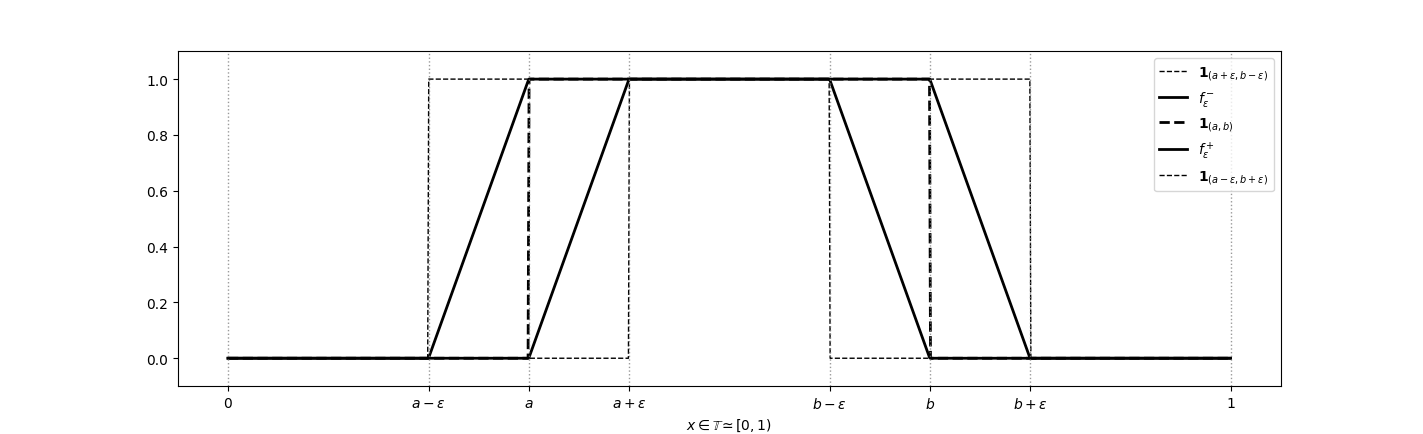
\includegraphics[scale=0.45]{pics/grafico_1_teorema_na.png}
        \caption{Gráfico de las funciones $\mathbf{1}_{(a+\varepsilon, b-\varepsilon)}$, 
        $f_\varepsilon^-$, $\mathbf{1}_{(a,b)}$, $f_\varepsilon^+$ y $\mathbf{1}_{(a-\varepsilon, b+\varepsilon)}$
        para el caso $(a,b) = (0.3, 0.7)$, $\varepsilon = 0.1$.}
    \end{figure}

    Sea $S_N = \sum_{n=1}^N \mathbf{1}_{(a,b)}(n\alpha)$, entonces,
    \[
        \frac{1}{N} \sum_{n=1}^N f_\varepsilon^-(n\alpha) \leq
        \frac{S_N}{N} \leq 
        \frac{1}{N} \sum_{n=1}^N f_\varepsilon^+(n\alpha)
    \]
    
    Por el lema anterior, se tiene que,
    \[
        b-a-2\varepsilon \leq
        \int_0^1 f_\varepsilon^-(x)\ dx \leq
        \liminf_{N \to \infty} \frac{S_N}{N} \leq
        \limsup_{N \to \infty} \frac{S_N}{N} \leq
        \int_0^1 f_\varepsilon^+(x)\ dx \leq
        b-a+2\varepsilon
    \]

    Finalmente, tomando el límite cuando $\varepsilon \to 0$ se obtiene,
    \[
        b-a \leq
        \liminf_{N \to \infty} \frac{S_N}{N} \leq
        \limsup_{N \to \infty} \frac{S_N}{N} \leq
        b-a
    \]

    Por lo tanto, el límite existe y
    \[
        \lim_{N \to \infty} \frac{1}{N} \sum_{n=1}^N \mathbf{1}_{(a,b)}(n\alpha) = b-a
    \]
\end{proof}






\chapter{Caracterizaciones de la equidistribución}
A continuación, presentamos dos herramientas fundamentales para el 
estudio de la equidistribución. La primera es una caracterización funcional,
que nos permite estudiar la equidistribución a través de las medias de
funciones integrables Riemann. La segunda es el criterio de Weyl, que proporciona 
una caracterización en términos de sumas exponenciales.  

\section{Caracterización funcional}

\begin{theorem}
    \label{carac:riemann}
    Sea $(x_n)_{n\geq1}$ una sucesión de números reales, entonces son equivalentes:
    \begin{enumerate}
        \item $(x_n)$ es equidistribuida módulo $1$.
        \item Para toda función $f\in \mathcal{R}(\mathbb{T})$, Riemann integrable, se cumple que
              \[
                  \lim_{N \to \infty} \frac{1}{N} \sum_{n=1}^N f(x_n) = \int_0^1 f(x)\ dx.
              \]
    \end{enumerate}
\end{theorem}

\begin{proof}
    $1 \Longrightarrow 2$ \, Sea $(x_n)$ una sucesión equidistribuida módulo 1.
    
    Consideremos la partición $0=a_0 < a_1 < \ldots < a_k=1$ de $\mathbb{T}$. Sea $f$ una función 
    escalonada tal que $f(x) = \sum_{i=1}^k c_i \mathbf{1}_{[a_{i-1}, a_i)}(x)$ con $c_i \in \mathbb{R}$
    para cada $i=1,\ldots,k$.

    Entonces,
    \[
        \frac{1}{N} \sum_{n=1}^N f(x_n) = 
        \frac{1}{N} \sum_{n=1}^N \sum_{i=1}^k c_i \mathbf{1}_{[a_{i-1}, a_i)}(x_n) = 
        \sum_{i=1}^k c_i \left(\frac{1}{N} \sum_{n=1}^N \mathbf{1}_{[a_{i-1}, a_i)}(x_n)\right)
    \]
    como $(x_n)$ es equidistribuida, por la observación~\ref{obs:equidistribucion}, 
    \begin{align*}
        \lim_{N \to \infty} \sum_{i=1}^k c_i \left(\frac{1}{N} \sum_{n=1}^N \mathbf{1}_{[a_{i-1}, a_i)}(x_n)\right)
        &= \sum_{i=1}^k c_i \left(\lim_{N \to \infty} \frac{1}{N} \sum_{n=1}^N \mathbf{1}_{[a_{i-1}, a_i)}(x_n)\right) \\
        &= \sum_{i=1}^k c_i \int_0^1 \mathbf{1}_{[a_{i-1}, a_i)}(x)\ dx \\
        &= \int_0^1 \sum_{i=1}^k c_i \mathbf{1}_{[a_{i-1}, a_i)}(x)\ dx 
        =\int_0^1 f(x)\ dx.
    \end{align*}
    
    Ahora, sea $f \in \mathcal{R}(\mathbb{T})$. Como $f$ es integrable Riemann, 
    para todo $\varepsilon > 0$ existe una partición $P=\{0=a_0<\cdots<a_k=1\}$ tal que, 
    si definimos
    \[
        L(x)=\sum_{i=1}^k m_i \mathbf{1}_{[a_{i-1},a_i)}(x) \qquad
        U(x)=\sum_{i=1}^k M_i \mathbf{1}_{[a_{i-1},a_i)}(x)
    \]
    donde $m_i=\inf_{x\in[a_{i-1},a_i)} f(x)$ y $M_i=\sup_{x\in[a_{i-1},a_i)} f(x)$
    se tiene
    \[
        L(x)\le f(x)\le U(x), \qquad \int_0^1 U(x) \, dx - \int_0^1 L(x) \, dx \leq \varepsilon.
    \]

    Sea $S_N = \sum_{n=1}^N f(x_n)$, tenemos,
    \[
        \frac{1}{N} \sum_{n=1}^N L(x_n) \leq \frac{S_N}{N} \leq \frac{1}{N} \sum_{n=1}^N U(x_n)
    \]
    como $L$ y $U$ son funciones escalonadas, al tomar límites,
    \[
        \int_0^1 f(x) \, dx - \varepsilon 
        \leq \int_0^1 L(x) \, dx 
        \leq \liminf_{N \to \infty} \frac{S_N}{N} 
        \leq \limsup_{N \to \infty} \frac{S_N}{N} 
        \leq \int_0^1 U(x) \, dx 
        \leq \int_0^1 f(x) \, dx + \varepsilon
    \]
    como $\varepsilon > 0$ es arbitrario, se concluye que
    \[
        \lim_{N \to \infty} \frac{1}{N} \sum_{n=1}^N f(x_n) = \int_0^1 f(x) \, dx.
    \]

    $2 \Longrightarrow 1$ \, Sea un intervalo $(a,b) \subset \mathbb{T}$ y sea $f(x) = \mathbf{1}_{(a,b)}(x)$, 
    como $f$ es Riemann integrable, entonces,
    \[
        \lim_{N \to \infty} \frac{1}{N} \sum_{n=1}^N \mathbf{1}_{(a,b)}(x_n) = \int_0^1 \mathbf{1}_{(a,b)}(x)\ dx = b-a
    \]

    lo que demuestra que $(x_n)$ es equidistribuida módulo $1$.
\end{proof}

\begin{corollary}
    \label{carac:continua}
    Sea $(x_n)_{n\geq1}$ una sucesión de números reales, entonces son equivalentes:
    \begin{enumerate}
        \item $(x_n)$ es equidistribuida módulo $1$.
        \item Para toda función $f\in C(\mathbb{T})$, se cumple que
              \[
                  \lim_{N \to \infty} \frac{1}{N} \sum_{n=1}^N f(x_n) = \int_0^1 f(x)\ dx.
              \]
    \end{enumerate}
\end{corollary}

\begin{example}
    Sea $(x_n)_{n\geq1}$ una sucesión en $\mathbb{T}$. Definimos $S((a,b),N) = \sum_{n=1}^N x_n \, \mathbf{1}_{(a,b)}(x_n)$
    donde $(a,b) \subseteq \mathbb{T}$. Entonces, la sucesión $(x_n)$ es equidistribuida módulo $1$ si y solo si 
    para todo intervalo $(a,b) \subseteq \mathbb{T}$
    \[
        \lim_{N \to \infty} \frac{S((a,b),N)}{N} = \frac{1}{2}(b^2-a^2)
    \]
\end{example}

\begin{proof}
    $\Longrightarrow$ \, Sea $(a,b) \subseteq \mathbb{T}$ y sea $f(x) = x \, \mathbf{1}_{(a,b)}(x)$.
    
    Como $f \in \mathcal{R}(\mathbb{T})$ y $(x_n)$ es equidistribuida,
    \[
        \lim_{N \to \infty} \frac{S((a,b),N)}{N} = 
        \lim_{N \to \infty} \frac{1}{N} \sum_{n=1}^N f(x_n) = 
        \int_0^1 f(x)\ dx = \int_a^b x\ dx = \frac{1}{2}(b^2-a^2)
    \]

    $\Longleftarrow$ \, 
    Vamos a probar que las CL de funciones $f(x)=x \, \mathbf{1}_{(a,b)}(x)$ son densas en $L^1(\mathbb{T})$.
    Para esto, sea $f \in L^1(\mathbb{T})$ y sea $\varepsilon > 0$. Por la densidad de las funciones simples, existe una función simple $s(x) = \sum_{i=1}^m a_i \mathbf{1}_{A_i}(x)$ tal que $\|f-s\|_1 < \varepsilon/2$.
    Dado que cada $A_i$ es medible, podemos aproximar cada $A_i$ por una unión finita de intervalos abiertos, es decir, existe una función $g(x) = \sum_{i=1}^m a_i \mathbf{1}_{B_i}(x)$ donde cada $B_i$ es una unión finita de intervalos abiertos tal que $\|s-g\|_1 < \varepsilon/2$.
    Por lo tanto, $\|f-g\|_1 \leq \|f-s\|_1 + \|s-g\|_1 < \varepsilon$.
    Finalmente, cada $B_i$ es una unión finita de intervalos abiertos, por lo que $g$ es una combinación lineal de funciones de la forma $x \, \mathbf{1}_{(a,b)}(x)$.      
\end{proof}

\section{El criterio de Weyl}

La caracterización funcional de la equidistribución es una herramienta de gran
utilidad, pero a menudo resulta difícil de aplicar a los distintos problemas. 
El criterio de Weyl proporciona un método más concreto para verificar la 
equidistribución, utilizando sumas exponenciales. 

Este criterio se basa en el hecho de que las funciones $f(x)=e^{2\pi i k x}$ con 
$k\in\mathbb{Z}$ son continuas y por tanto, satisfacen las condiciones
del corolario \ref{carac:continua}. Además, esta familia de funciones es lo suficientemente 
rica como para caracterizar la equidistribución.

\begin{theorem}
    \label{teo:criterio_weyl}
    Sea $(x_n)$ una sucesión en $[0,1)$, entonces son equivalentes:
    \begin{enumerate}
        \item $(x_n)$ es equidistribuida en $[0,1)$.
        \item Para todo $k \in \mathbb{Z} \setminus \{0\}$,
              \[
                  \frac{1}{N} \sum_{n=1}^N e^{2\pi i k x_n} \longrightarrow 0 \quad \text{cuando } N \to \infty.
              \]
    \end{enumerate}
\end{theorem}

\begin{proof}
    $1 \Longrightarrow 2$ \, Sea $k \in \mathbb{Z} \setminus \{0\}$, como $(x_n)$ es equidistribuida aplicando
    el teorema anterior a la función $f(x) = e^{2\pi i k x}$, entonces,
    \[
        \lim_{N \to \infty} \frac{1}{N} \sum_{n=1}^N e^{2\pi i k x_n} = \int_0^1 e^{2\pi i k x}\ dx = 0.
    \]
    $2 \Longrightarrow 1$ \, La hipótesis es el paso $2$ del Lema \ref{lem:lema_na}. Reproduciendo la prueba,
    se concluye que $(x_n)$ es equidistribuida módulo $1$. 
\end{proof}


\begin{example}
    La sucesión $(n\alpha)_{n\geq1}$ con $\alpha \notin \mathbb{Q}$ es equidistribuida módulo $1$.
\end{example}

\begin{resolve}
    Sea $k \in \mathbb{Z}\setminus\{0\}$,
    \[
        \left|\frac{1}{N}\sum_{n=1}^N e^{2\pi i k n\alpha} \right| =
        \frac{1}{N} \left|\frac{e^{2\pi i k \alpha}(1-e^{2\pi i k N \alpha})}{1-e^{2\pi i k \alpha}} \right| \leq
        \frac{2}{N|e^{2\pi i k \alpha}-1|}
    \]
    Como $\alpha \notin \mathbb{Q}$, se tiene $k\alpha \notin \mathbb{Z}$ y por tanto $e^{2\pi i k \alpha} \neq 1$
    
    Al tomar el límite cuando $N \to \infty$ se concluye que
    \[
        \lim_{N \to \infty} \frac{1}{N}\sum_{n=1}^N e^{2\pi i k n\alpha} = 0
    \]
    y por el criterio de Weyl, la sucesión $(n\alpha)$ es equidistribuida módulo $1$.
\end{resolve}



\begin{example} 
    \label{ex:ax-b}
    Sea $(x_n)_{n\geq1}$ una sucesión equidistribuida módulo $1$, sea $a\in \mathbb{Z}\setminus\{0\}$ y sea $b\in\mathbb{R}$.
    Entonces la sucesión $(ax_n+b)_{n\geq1}$ es equidistribuida módulo $1$.
\end{example}

\begin{resolve}
    Definimos $y_n = ax_n+b$. Para cada $k \in \mathbb{Z}\setminus\{0\}$ se tiene
    \[
        \left|\frac{1}{N}\sum_{n=1}^N e^{2\pi i k y_n} \right|
        = \left|\frac{1}{N}\sum_{n=1}^N e^{2\pi i k (ax_n + b)} \right|
        = \left|\frac{1}{N}e^{2\pi i k b}\sum_{n=1}^N e^{2\pi i (ka) x_n} \right|
        =\left|\frac{1}{N}\sum_{n=1}^N e^{2\pi i (ka) x_n} \right|.
    \]
    
    Dado que $ka \in \mathbb{Z}\setminus\{0\}$ y $(x_n)$ es equidistribuida, el criterio de Weyl implica que
    \[
        \lim_{N\to\infty} \frac{1}{N}\sum_{n=1}^N e^{2\pi i (ka) x_n} = 0.
    \]
    
    Por consiguiente,
    \[
        \lim_{N\to\infty} \frac{1}{N}\sum_{n=1}^N e^{2\pi i k y_n}  = 0.
    \]
    y por el criterio de Weyl, la sucesión $(y_n)$ es equidistribuida módulo $1$.
\end{resolve}

Como consecuencia, la proposición \ref{prop:secuencia_mas_const} es un corolario de este resultado.

\begin{example}
    La sucesión $\partfrac{\sin n}$ es densa en $[0,1)$ pero no es equidistribuida.
\end{example} 

\begin{resolve}
    Sabemos que $n$ es equidistribuida en $[0,2\pi)$.
    Por la caracterización funcional de la equidistribución aplicada a la función $f(x) = e^{2\pi i \sin x}$, tenemos que
    \[
        \frac{1}{N} \sum_{n=1}^N e^{2\pi i \sin n} \longrightarrow \frac{1}{2\pi} \int_0^{2\pi} e^{2\pi i \sin x} dx \qquad \text{cuando } N \to \infty.
    \]

    Si calculamos esta integral, tenemos que
    \[
        \int_0^{2\pi} e^{2\pi i \sin x} dx = 2\pi J_0(2\pi) \neq 0.
    \]

    Si $\partfrac{\sin n}$ fuese equidistribuida, por el criterio de Weyl, debería cumplirse
    \[
        \forall \, k \in \mathbb{Z}\setminus\{0\}, \quad \frac{1}{N} \sum_{n=1}^N e^{2\pi i k \sin n} \longrightarrow 0 \qquad \text{cuando } N \to \infty,
    \]
    Pero para $k=1$ hemos visto que esta suma tiende a $J_0(2\pi) \neq 0$, lo que demuestra que $\partfrac{\sin n}$ no es equidistribuida.
\end{resolve}



\chapter{Método de Euler}
Mediante el criterio de Weyl, podemos demostrar facilmente que una sucesión es equidistribuida.
En este capítulo presentamos un método, inspirado en los ejercicios de Kuipers 
\cite[Ejercicios 2.21--2.22]{kuipers-1974}, para verificar dicha propiedad apoyándose en la fórmula de sumación de Euler. 

Esta fórmula nos permite expresar sumas de exponenciales en términos de integrales, las
cuales podemos acotar de forma precisa.


\begin{proposition}[Fórmula de sumación de Euler]
    Sea $N \in \mathbb{N}$ y sea $f:[1,N] \to \mathbb{C}$ una función tal que $f' \in C([1,N])$. 
    Entonces se cumple la siguiente igualdad:
    \begin{align}
        \label{prop:formula_euler}
        \sum_{n=1}^N f(n) = 
        \int_1^N f(x) \, dx + 
        \frac{f(1)+f(N)}{2} + 
        \int_1^N \left(\partfrac{x} - \frac{1}{2}\right) \, f'(x) \, dx
    \end{align}
\end{proposition}

\begin{proof}
    Dividimos el intervalo $[1,N]$ en subintervalos $[n,n+1]$ con $n=1,\ldots,N-1$. 
    
    Para cada intervalo $[n,n+1]$ se tiene que $\partfrac{x} = x - n$, 
    al integrar por partes,
    \begin{align*} 
        \int_n^{n+1} \left(\partfrac{x} - \frac{1}{2}\right) f'(x) \, dx 
        &= \left[\left(\partfrac{x} - \frac{1}{2}\right) f(x) \right]_n^{n+1} - \int_n^{n+1} f(x) \, dx \\
        &= \frac{1}{2} \, f(n+1) + \frac{1}{2} \, f(n) - \int_n^{n+1} f(x) \, dx
    \end{align*}

    Sumando sobre $n=1,2,\ldots,N-1$,
    \[
        \sum_{n=1}^{N-1} \int_n^{n+1} \left(\partfrac{x} - \frac{1}{2}\right) \, f'(x) \, dx =
        \sum_{n=1}^{N-1} \left(\frac{1}{2} \, f(n+1) + \frac{1}{2} \, f(n)\right) -
        \sum_{n=1}^{N-1} \int_n^{n+1} f(x) \, dx \\
    \]
    luego,
    \[
        \int_1^N \left(\partfrac{x} - \frac{1}{2}\right) \, f'(x) \, dx =
        \sum_{n=1}^N f(n) - \frac{1}{2} \, f(N) - \frac{1}{2} \, f(1) - 
        \int_1^N f(x) \, dx
    \]
    
    Reordenando los términos se obtiene la igualdad deseada.
\end{proof}

\begin{example}
    La sucesión $(a\log n)_{n\geq1}$ con $a \in \mathbb{R}$ no es equidistribuida módulo $1$.
\end{example}

\begin{resolve}
    Si $a = 0$, la secuencia es constante e igual a $0$, por lo que no es equidistribuida.
    
    Supongamos que $a \neq 0$. Verificaremos que no se cumple el criterio de Weyl para $k=1$. 
    Es decir,
    \[
        \lim_{N \to \infty} \frac{1}{N} \sum_{n=1}^N e^{2\pi i a \log n} \neq 0
    \]   
    
    Sea $f(x) = e^{2\pi i a \log x}$. Aplicando la fórmula (\ref{prop:formula_euler})
    \[
        \sum_{n=1}^N e^{2\pi i \, a \log n} =
        \int_1^N e^{2\pi i a \log x} \, dx +
        \frac{1}{2} \left(e^{2\pi i \, a \log N} + 1\right) +
        \int_1^N \left(\partfrac{x} - \frac{1}{2}\right) \frac{2\pi i a}{x} \, e^{2\pi i a \log x} \, dx 
    \]
    
    Calculamos la primera integral mediante el cambio de variable $u = \log x$,
    $x = e^u$ y $dx = e^u du$. Cuando $x = 1$, $u = 0$ y cuando $x = N$, $u = \log N$.
    \begin{align*}
        \int_1^N e^{2\pi i a \log x} \, dx 
        = \int_0^{\log N} e^{(2\pi i a + 1) u} \, du 
        &= \left[\frac{e^{(2\pi i a + 1) u}}{2\pi i a + 1}\right]_0^{\log N} \\ 
        &= \frac{e^{(2\pi i a + 1) \log N} - 1}{2\pi i a + 1} 
        = \frac{N e^{2\pi i a \log N} - 1}{2\pi i a + 1}
    \end{align*}
        
    Dividiendo por $N$, 
    \[
        \frac{N e^{2\pi i a \log N} - 1}{N(2\pi i a + 1)}
        = \frac{e^{2\pi i a \log N}}{2\pi i a + 1} - \frac{1}{N(2\pi i a + 1)}
    \]

    Cuando $N \to \infty$, el segundo término se anula, mientras que el primero 
    no converge, ya que oscila sobre la circunferencia unidad.

    El término central se puede acotar
    \[
        \left|\frac{1}{2} \left(e^{2\pi i a \log N} + 1\right)\right| \leq 1
    \]
    por lo que, tras dividir por $N$, támbien tiende a $0$.

    Para la segunda integral, usamos que $|\partfrac{x} - \frac{1}{2}| \leq \frac{1}{2}$ y que $|e^{2\pi i a \log x}| = 1$,
    \[
        \left|\int_1^N \left(\partfrac{x} - \frac{1}{2}\right) \dfrac{2\pi i a}{x} \, e^{2\pi i a \log x} \, dx\right|
        \leq \pi |a| \int_1^N \frac{1}{x} \, dx
        = \pi |a| \log N
    \]
    En consecuencia,
    \[
        \frac{1}{N} \left|\int_1^N \left(\partfrac{x} - \frac{1}{2}\right) \dfrac{2\pi i a}{x} \, e^{2\pi i a \log x} \, dx\right|
        \longrightarrow 0 \qquad \text{cuando} \ N \to \infty
    \]

    Como la primera integral no tiende a $0$, no se verifica el criterio de Weyl para $k=1$.
    Por tanto, la sucesión $(a\log n)$ no es equidistribuida módulo $1$.   
\end{resolve}


\begin{example}
    La sucesión $(an^\sigma)_{n\geq1}$ con $a \in \mathbb{R}$, $a \neq 0$ y 
    $\sigma \in (0,1)$ es equidistribuida módulo $1$.
\end{example}

\begin{resolve}    
    Para demostrarlo utilizaremos el criterio de Weyl. 

    Sea $k \in \mathbb{Z}\setminus\{0\}$, como $a \neq 0$, entonces $b = ak \neq 0$. 
    Basta comprobar que 
    \[
        \frac{1}{N} \sum_{n=1}^N e^{2\pi i b n^\sigma} \longrightarrow 0 
        \qquad \text{cuando} \ N \to \infty.
    \]

    Aplicando la fórmula (\ref{prop:formula_euler}) a la función $f(x) = e^{2\pi i b x^\sigma}$,
    \[
        \sum_{n=1}^N e^{2\pi i \, b n^\sigma}
        = \int_1^N e^{2\pi i b x^\sigma} \, dx 
        + \frac{1}{2} \left(e^{2\pi i \, b N^\sigma} + e^{2\pi i b}\right)
        + \int_1^N \left(\partfrac{x} - \frac{1}{2}\right) 2\pi i b \sigma x^{\sigma-1} \, e^{2\pi i b x^\sigma} \, dx 
    \]

    Calculamos la primera integral usando integración por partes,
    \begin{align*}
        \int_1^N e^{2\pi i b x^\sigma} \, dx 
        = \int_1^N \frac{\left(e^{2\pi i b x^\sigma}\right)'}{2\pi i b \sigma x^{\sigma-1}} \, dx
        &= \frac{1}{2 \pi i b \sigma} \int_1^N \left(e^{2\pi i b x^\sigma}\right)'x^{1-\sigma} \, dx \\
        &= \frac{1}{2 \pi i b \sigma} \left(\left[e^{2\pi i b x^\sigma}x^{1-\sigma}\right]_1^N + (1-\sigma) \int_1^N e^{2\pi i b x^\sigma} x^{-\sigma} \, dx \right)
    \end{align*}  
    
    Acotando cada uno de los términos anteriores,
    \begin{align*}
        \left| e^{2\pi i b N^\sigma}N^{1-\sigma} - e^{2\pi i b}\right|
        &\leq N^{1-\sigma} + 1 \\
        \left|\int_1^N e^{2\pi i b x^\sigma} x^{-\sigma} \, dx\right|
        &\leq \int_1^N x^{-\sigma} \, dx
        = \frac{N^{1-\sigma} - 1}{1-\sigma}
    \end{align*}
    Ambos crecen del orden de $N^{1-\sigma}$, por lo que la primera integral es$O(N^{1-\sigma})$.

    El término central se acota por
    \[
        \left|\frac{1}{2} \left(e^{2\pi i b N^\sigma} + e^{2\pi i b}\right)\right| \leq 1
    \]
    luego es $O(1)$.

    Para la segunda integral, usando que $|\partfrac{x} - \frac{1}{2}| \leq \frac{1}{2}$,
    y que $|e^{2\pi i b x^\sigma}| = 1$, se tiene
    \[
        \left|\int_1^N \left(\partfrac{x} - \frac{1}{2}\right) 2\pi i b \sigma x^{\sigma-1} \, e^{2\pi i b x^\sigma} \, dx\right|
        \leq \pi |b| \int_1^N \sigma x^{\sigma-1} \, dx  
        = \pi |b| (N^\sigma - 1)
    \]
    por lo que esta integral es $O(N^\sigma)$.
    
    Reuniendo las estimaciones anteriores, y teniendo en cuenta que 
    $\sigma \in (0,1)$, se obtiene
    \[
        \sum_{n=1}^N e^{2\pi i \, b n^\sigma} = O(N^{1-\sigma}) + O(1) + O(N^\sigma) = O(N^{\max\{\sigma, 1-\sigma\}}) = o(N)
    \]
    De este modo,
    \[
        \frac{1}{N} \sum_{n=1}^N e^{2\pi i b n^\sigma} \longrightarrow 0 
        \qquad \text{cuando} \ N \to \infty,
    \]
    y por tanto la sucesión $(an^\sigma)$ es equidistribuida módulo $1$.
\end{resolve}



La idea del ejemplo anterior se puede extender a funciones más generales que cumplan 
ciertas condiciones de crecimiento. El siguiente resultado, el teorema de Fejér, 
nos dice con precisión cuáles son estas condiciones.

    Mediante la fórmula de sumación de Euler (\ref{prop:SumacionEuler}), sea $f(x) = e^{2\pi i k g(x)}$ y sea $k \in \mathbb{Z} \setminus \{0\}$.
    Veamos que condiciones debe cumplir $g$ para que se cumpla el criterio de Weyl.
    \[
        \sum_{n=1}^N e^{2\pi i k g(n)}
        = \int_1^N e^{2\pi i k g(x)} \, dx 
        + \frac{1}{2} \left(e^{2\pi i k g(N)} + e^{2\pi i k g(1)}\right)
        + \int_1^N \left(\partfrac{x} - \frac{1}{2}\right) 2\pi i k g'(x) \, e^{2\pi i k g(x)} \, dx
    \]

    La primera integral la calculamos usando integración por partes.
    \begin{align*}
        \int_1^N e^{2\pi i k g(x)} \, dx 
        = \int_1^N \frac{\left(e^{2\pi i k g(x)}\right)'}{2\pi i k g'(x)} \, dx
        &= \frac{1}{2 \pi i k} \int_1^N \frac{\left(e^{2\pi i k g(x)}\right)'}{g'(x)} \, dx \\
        &= \frac{1}{2 \pi i k} \left(\left[\frac{e^{2\pi i k g(x)}}{    g'(x)}\right]_1^N + \int_1^N e^{2\pi i k g(x)} \left(\frac{1}{g'(x)}\right)' \, dx \right)
    \end{align*}
    Vamos a ver cada termino por separado.
    \begin{align*}
        \left|\frac{e^{2\pi i k g(N)}}{g'(N)} - \frac{e^{2\pi i k g(1)}}{g'(1)}\right|
        &\leq \frac{1}{|g'(N)|} + \frac{1}{|g'(1)|} \\
        \left|\int_1^N e^{2\pi i k g(x)}\left(\frac{1}{g'(x)}\right)' \, dx\right|
        \leq \int_1^N \left|\left(\frac{1}{g'(x)}\right)' \right| \, dx 
        &= \left|\frac{1}{g'(N)} - \frac{1}{g'(1)}\right|
        \leq \frac{1}{|g'(N)|} + \frac{1}{|g'(1)|}
    \end{align*}
    Por la monotonia de $g'$ podemos quitar el valor absoluto de la integral
    Por lo tanto, sea $C_1$ una constante que amontone las cotas todo lo que no depende de $N$.
    \[
        \left|\frac{1}{N} \int_{1}^N e^{2\pi i k g(n)}\right| \leq \frac{C_1}{N \left|g'(x)\right|}
    \]
    Necesitamos que se cumpla la condicion $\lim_{x \to \infty} {x \left|g'(x)\right|} = \infty$

    El termino central se puede acotar por $1$, no necesitamos nada especial para él.

    La última integral se puede acotar usando que $|\partfrac{x} - \frac{1}{2}| \leq \frac{1}{2}$, $|e^{2\pi i k g(x)}| = 1$ y por lo tanto
    \[
        \left|\int_1^N \left(\partfrac{x} - \frac{1}{2}\right) 2\pi i k g'(x) \, e^{2\pi i k g(x)} \, dx\right|
        \leq \int_1^N \frac{1}{2} \, 2\pi |k| |g'(x)| \, dx
        = \pi |k| (g(N) - g(1))
    \]
    Aglutinando todo en otra constante $C_2$ que amontone las cotas todo lo que no depende de $N$,
    \[
        \left|\frac{1}{N} \int_1^N \left(\partfrac{x} - \frac{1}{2}\right) 2\pi i k g'(x) \, e^{2\pi i k g(x)} \, dx\right| \leq C_2 \left|\frac{g(N)}{N}\right|
    \]
    Necesitamos que se cumpla la condición $\lim_{x \to \infty} \frac{g(x)}{x} = 0$.

\begin{example}
    Las sucesiones $(an^\sigma\log^\tau n)_{n\geq2}$ con $a \neq 0$, 
    $\sigma \in (0,1)$ y $\tau \in \mathbb{R}$ son equidistribuidas módulo $1$.
\end{example}

\begin{resolve}
    Sea $x_n = an^\sigma\log^\tau n$ para cada $n \geq 2$. Definimos $g(x) = a(x+1)^\sigma\log^\tau (x+1)$
    en~$[1,\infty)$, entonces $g(n) = x_{n+1}$ para cada $n \geq 1$, y su derivada es 
    \[
        g'(x) = a (x+1)^{\sigma-1} \log^{\tau-1}(x+1) \left(\sigma \log(x+1) + \tau\right)
    \]
    esta es continua en $[1,\infty)$ por ser composición de continuas y como $\sigma \in (0,1)$, 
    \[
        \lim_{x \to \infty} g'(x) = 0
        \qquad \text{y} \qquad
        \lim_{x \to \infty} x |g'(x)| = \infty
    \]

    Monotonia, estudiar como hacerlo.

    Por el teorema \ref{teo:fejer_euler}, $(g(n))$ es equidistribuida módulo $1$ y 
    por lo tanto, $(x_n)$ también lo es.
\end{resolve}

\begin{example}
    Las sucesiones $(a\log^\tau n)_{n\geq1}$ con $a \neq 0$ y $\tau > 1$ son equidistribuidas módulo $1$.
\end{example}

\begin{resolve}
    Sea $g(x) = a\log^\tau (x)$ entonces su derivada es
    \[
        g'(x) = \frac{a \tau \log^{\tau-1}(x)}{x}
    \]
    como $\tau > 1$, es continua en $[1,\infty)$ por ser composición de continuas. Además, 
    \[
        \lim_{x \to \infty} g'(x) = 0
        \qquad \text{y} \qquad
        \lim_{x \to \infty} x |g'(x)| = \infty
    \]

    Para ver la monotonía de $g'(x)$, calculamos su derivada,
    \[
        g''(x) = a \tau \frac{\log^{\tau-2}(x)}{x^2} \left((\tau - 1) - \log(x)\right)
    \]
    Obtenemos que $g''(x)=0$ en $x = e^{\tau - 1}$, por lo que, para $x > e^{\tau - 1}$ tendremos que
    $g''(x)$ es de signo constante. Luego $g'(x)$ es monótona a partir de $x_0 = e^{\tau - 1}$.

    Por el teorema \ref{teo:fejer_euler}, la sucesión $(a\log^\tau (n))$ es equidistribuida módulo $1$.
\end{resolve}

\begin{example}
    Las sucesiones $(an\log^\tau n)_{n\geq2}$ con $a \neq 0$ y $\tau < 0$ son equidistribuidas módulo $1$.
\end{example}

\begin{resolve}
    Sea $x_n = an\log^\tau n$ para cada $n \geq 2$. Definimos $g(x) = a(x+1)\log^\tau (x+1)$
    en~$[1,\infty)$, entonces $g(n) = x_{n+1}$ para cada $n \geq 1$, y su derivada es 
    \[
        g'(x) = a \log^{\tau}(x+1) + a \tau \log^{\tau-1}(x+1)
    \]
    que es continua en $[1,\infty)$ por ser composición de continuas y como $\tau < 0$, 
    \[
        \lim_{x \to \infty} g'(x) = 0
        \qquad \text{y} \qquad
        \lim_{x \to \infty} x |g'(x)| = \infty
    \]

    Para comprobar la monotonía de $g'(x)$, calculamos su derivada,
    \[
        g''(x) = a \tau \frac{\log^{\tau-2}(x+1)}{x+1} \left(\log(x+1) + \tau - 1\right)
    \]
    Como $g''(x)=0$ en $x = e^{1-\tau} - 1$, entonces para $x \geq e^{1-\tau} - 1$ 
    se tiene que $g''(x)$ es de signo constante. En consecuencia, $g'(x)$ es monótona a 
    partir de $x_0 = e^{1-\tau} - 1$.

    Por el teorema \ref{teo:fejer_euler}, $(g(n))$ es equidistribuida módulo $1$ y 
    por lo tanto, $(x_n)$ también lo es.
\end{resolve}

\chapter{Método de Van der Corput}
\section{Desigualdad de Van der Corput}

\begin{lemma}[Desigualdad de Van der Corput]
    \label{lem:vandercorput}
    Sean $H,N \in \mathbb{N}$ con $1 \leq H \leq N$ entonces,
    \begin{align}
        \left| \sum_{n=1}^N e^{2\pi i f(n)} \right|^2 \leq
        4 \, \frac{N}{H} \sum_{h=0}^{H-1} \left| \sum_{n=1}^{N-h} e^{2\pi i (f(n+h) - f(n))} \right|
    \end{align}
\end{lemma}

\begin{proof}
    Sea $u_n \in \mathbb{C}$ con $n = 1, \dots, N$. Definimos $u_n = 0$ para $n > N$ y 
    para $n \leq 0$. Entonces,
    \[
        H \sum_{n=1}^{N} u_n = \sum_{k=1}^{H} \sum_{n=1}^{N} u_n
    \]
    Sea $k$ fijo, consideramos el cambio de variable $p = n+k$ entonces $n = p-k$ y $p=1+k,\dots,N+k$
    \[
        \sum_{k=1}^{H} \sum_{n=1}^{N} u_n =
        \sum_{k=1}^{H} \sum_{p=k+1}^{N+k} u_{p-k}
    \]
    Por lo tanto, gracias a la extensión de ceros de los $u_n$,
    \[
        H \sum_{n=1}^{N} u_n =
        \sum_{k=1}^{H} \sum_{p=2}^{N+H} u_{p-k} =
        \sum_{p=2}^{N+H} \sum_{k=1}^{H} u_{p-k}
    \]
    
    Ahora elevamos al cuadrado ambos lados y aplicamos la desigualdad de Cauchy-Schwarz, \ref{ap:cauchy-schwarz},
    \[
        \left| H \sum_{n=1}^{N} u_n \right|^2 \leq
        (N+H-1) \sum_{p=2}^{N+H} \left| \sum_{k=1}^{H} u_{p-k} \right|^2
    \]
    
    Fijado $p$, vamos a desarrollar el sumatorio de dentro del término de la derecha,
    \[
        \left|  \sum_{k=1}^{H} u_{p-k} \right|^2 =
        \left(\sum_{k=1}^{H} u_{p-k} \right)\left( \sum_{s=1}^{H} \overline{u_{p-s}} \right) =
        \sum_{k=1}^{H} \sum_{s=1}^{H} u_{p-k} \overline{u_{p-s}}
    \]
    Este doble sumatorio se descompone en tres partes, la primera es la parte diagonal $k=s$,
    la segunda es la parte inferior $k < s$ y la tercera es la parte superior $k > s$,
    \[
        \sum_{k=1}^{H} \sum_{s=1}^{H} u_{p-k} \overline{u_{p-s}} =
        \sum_{k=1}^{H} |u_{p-k}|^2 \, +
        \sum_{1 \leq k < s \leq H} u_{p-k} \overline{u_{p-s}} \, +
        \sum_{1 \leq s < k \leq H} u_{p-k} \overline{u_{p-s}}
    \]
    Gracias a la simetría de los sumatorios de la parte inferior e superior,
    se pueden juntar ambos sumatorios y se obtiene,
    \[
        \sum_{k=1}^{H} \sum_{s=1}^{H} u_{p-k} \overline{u_{p-s}} =
        \sum_{k=1}^{H} |u_{p-k}|^2 \, +
        \sum_{1 \leq k < s \leq H} 2\operatorname{Re}(u_{p-k} \overline{u_{p-s}})
    \]

    De momento tenemos la siguiente cota,
    \begin{align*}
        H^2 \left| \sum_{n=1}^{N} u_n \right|^2 
        &\leq (N+H-1) \sum_{p=2}^{N+H} \sum_{k=1}^{H} |u_{p-k}|^2 +
        2(N+H-1) \sum_{p=2}^{N+H} \sum_{1 \leq k < s \leq H} \operatorname{Re}(u_{p-k} \overline{u_{p-s}}) \\
        &\leq (N+H-1) H \sum_{n=1}^{N} |u_{n}|^2 +
        2(N+H-1) \operatorname{Re}\left(\sum_{p=2}^{N+H} \sum_{1 \leq k < s \leq H} u_{p-k} \overline{u_{p-s}}\right)
    \end{align*}

    Estudiamos sumatorio del segundo término. Hacemos el cambio de variable $n = p-s$,
    notando que $u_n = 0$ salvo para $n=1,\dots,N$. Además, como la suma es finita podemos
    cambiar el orden de los sumatorios,
    \[
        \sum_{p=2}^{N+H} \sum_{1 \leq k < s \leq H} u_{p-k} \overline{u_{p-s}} =
        \sum_{1 \leq k < s \leq H} \sum_{n=1}^{N} u_{n+s-k} \overline{u_n}
    \]
    Sea $k$ fijo, hacemos el cambio de variable $h = s-k$. Como $k < s$ entonces 
    $s = k+1, \dots, H$ y $h = 1, \dots, H-k$. Obtenemos,
    \[
        \sum_{1 \leq k < s \leq H} \sum_{n=1}^{N} u_{n+s-k} \overline{u_n} =
        \sum_{k=1}^{H-1} \sum_{h=1}^{H-k} \sum_{n=1}^{N} u_{n+h} \overline{u_n}
    \]
    Sabemos que $1 \leq h \leq H-k$ entonces $2 \leq h+k \leq H$ y $1 \leq k \leq H-h$,
    \begin{align*}
        \sum_{k=1}^{H-1} \sum_{h=1}^{H-k} \sum_{n=1}^{N} u_{n+h} \overline{u_n}  
        &=\sum_{k=1}^{H-1} \sum_{h=1}^{H-1} \mathbf{1}_{[2,H]}(h+k) \left(\sum_{n=1}^{N} u_{n+h} \overline{u_n} \right) \\
        &=\sum_{h=1}^{H-1} \sum_{k=1}^{H-1} \mathbf{1}_{[2,H]}(h+k) \left(\sum_{n=1}^{N} u_{n+h} \overline{u_n} \right) \\
        &=\sum_{h=1}^{H-1} \sum_{k=1}^{H-h} \left(\sum_{n=1}^{N} u_{n+h} \overline{u_n} \right) \\
        &=\sum_{h=1}^{H-1} (H-h) \left(\sum_{n=1}^{N} u_{n+h} \overline{u_n} \right)
     \end{align*}

     La cota que teníamos la podemos simplificar como,
     \begin{align*}
        H^2 \left| \sum_{n=1}^{N} u_n \right|^2 
        &\leq (N+H-1) H \sum_{n=1}^{N} |u_{n}|^2 + 2(N+H-1) \operatorname{Re}\left(\sum_{h=1}^{H-1} (H-h) \left(\sum_{n=0}^{N} u_{n+h} \overline{u_n} \right)\right) \\        
        &\leq 2(N+H-1) \operatorname{Re}\left(\sum_{h=0}^{H-1} (H-h) \left(\sum_{n=0}^{N} u_{n+h} \overline{u_n} \right)\right) 
    \end{align*}

    Considerando las siguientes cotaciones $N+H-1 \leq 2N$, $H-h \leq H$ y 
    $\operatorname{Re}(z) \leq |z|$ para todo $z \in \mathbb{C}$ y teniendo en cuenta
    que $u_n=0$ salvo para $n=1,\dots,N$ obtenemos,
    \[
        H^2 \left| \sum_{n=1}^{N} u_n \right|^2 \leq
        4N H \sum_{h=0}^{H-1} \left| \sum_{n=1}^{N-h} u_{n+h} \overline{u_n} \right|
    \]

    Finalmente, dividiendo ambos lados por $H^2$ y aplicando $u_n = e^{2\pi i f(n)}$ 
    obtenemos la fórmula deseada,
    \[
        \left| \sum_{n=1}^N e^{2\pi i f(n)} \right|^2 \leq
        4 \, \frac{N}{H} \sum_{h=0}^{H-1} \left| \sum_{n=1}^{N-h} e^{2\pi i (f(n+h) - f(n))} \right|
    \]
\end{proof}

\section{Teorema de las diferencias de Van der Corput}

\begin{example}
    La sucesión $\partfrac{n^2\alpha}$ con $\alpha \notin \mathbb{Q}$ es equidistribuida en $[0,1)$.
\end{example}

\begin{resolve}
    Sea $f(n)=n^2\alpha$ con $\alpha \notin \mathbb{Q}$, entonces
    \[
        f(n+h)-f(n)=n^2\alpha + 2nh\alpha + h^2\alpha - n^2\alpha = 2nh\alpha+h^2\alpha.
    \]

    Usando la estimación anterior, como para $h=0$ se tiene $e^{2\pi i 0}=1$, entonces
    \[
        \left|\sum_{n=1}^N e^{2\pi i  k n^2 \alpha}\right|^2 \leq 
        4\,\frac{N^2}{H} + 4\,\frac{N}{H} \sum_{h=1}^{H-1} \left|\sum_{n=1}^{N-h} e^{2\pi i k (2nh\alpha+h^2\alpha)}\right|.
    \]

    Para cada $h \neq 0$, por el ejemplo \ref{ex:ax-b}, se tiene que $\partfrac{2nh\alpha+h^2\alpha}$ es equidistribuida en $[0,1)$.

    Al dividir por $N^2$,
    \[
        \left|\frac{1}{N}\sum_{n=1}^N e^{2\pi i n^2 \alpha}\right|^2 \leq 
        \frac{4}{H} + \frac{4}{N} \sum_{h=1}^{H-1} \frac{N-h}{N} \left|\frac{1}{N-h}\sum_{n=1}^{N-h} e^{2\pi i k(2nh\alpha+h^2\alpha)}\right|.
    \]

    Fijado $H$, por el criterio de Weyl, para cada $h \neq 0$ se tiene que
    \[
        \lim_{N\to\infty} \frac{1}{N-h}\sum_{n=1}^{N-h} e^{2\pi i k(2nh\alpha+h^2\alpha)} = 0.
    \] 

    Luego,
    \[
        \limsup_{N\to\infty} \left| \frac{1}{N} \sum_{n=1}^N e^{2\pi i k n^2 \alpha}\right|^2 \leq \frac{4}{H}.
    \]  

    Dado que es cierto para cada $H\in \mathbb{N}$, haciendo $H\to\infty$ se concluye que
    \[
        \lim_{N\to\infty} \left| \frac{1}{N} \sum_{n=1}^N e^{2\pi i k n^2 \alpha}\right|^2 = 0.
    \]
    
    Por lo tanto, por el criterio de Weyl, la sucesión $\partfrac{n^2\alpha}$ es equidistribuida en $[0,1)$.
\end{resolve}

\begin{theorem}[Teorema de las diferencias de Van der Corput]
    \label{teo:diferencias_weyl}
    Sea $(x_n)_{n\geq1}$ una sucesión de números reales. Si para cada $h=1,2,\dots,$
    la sucesión $(x_{n+h}-x_n)$ es equidistribuida módulo $1$, entonces la sucesión
    $(x_n)$ es equidistribuida módulo $1$.
\end{theorem}

\begin{proof}
    Sea $k\in \mathbb{Z}\setminus\{0\}$ y sea $f(n)=kx_n$, usando la estimación 
    (\ref{lem:vandercorput}), y teniendo en cuenta que para $h=0$ se tiene $e^{2\pi i 0}=1$.
    Obtenemos
    \[
        \left|\frac{1}{N}\sum_{n=1}^N e^{2\pi i k x_n}\right|^2 \leq
        \frac{4}{H} + \frac{4}{H} \sum_{h=1}^{H-1} \frac{N-h}{N} \left|\frac{1}{N-h}\sum_{n=1}^{N-h} e^{2\pi i k (x_{n+h}-x_n)} \right|
    \]

    Dado que para cada $h=1,2,\dots,$ la sucesión $(x_{n+h}-x_n)$ es equidistribuida módulo $1$,
    por el criterio de Weyl se tiene que
    \[
        \lim_{N\to\infty} \frac{1}{N-h}\sum_{n=1}^{N-h} e^{2\pi i k (x_{n+h}-x_n)} = 0.
    \]
    Luego,
    \[
        \limsup_{N\to\infty} \left|\frac{1}{N}\sum_{n=1}^N e^{2\pi i k x_n}\right|^2 \leq \frac{4}{H}.
    \]
    
    Dado que es cierto para cada $H\in \mathbb{N}$, haciendo $H\to\infty$ se concluye que
    \[
        \lim_{N\to\infty} \left|\frac{1}{N}\sum_{n=1}^N e^{2\pi i k x_n}\right|^2 = 0.
    \]

    Por lo tanto, por el criterio de Weyl, la sucesión $(x_n)$ es equidistribuida módulo $1$.
\end{proof}
    

\section{Aplicaciones del teorema de las diferencias}

\begin{theorem}
    \label{teo:polinomios_weyl}
    Sea $p(x)=c_m x^m + c_{m-1} x^{m-1} + \dots + c_1 x + c_0$ un polinomio con coeficientes 
    reales. Si al menos uno de $c_j \notin \mathbb{Q}$ con $j>0$, entonces la sucesión $(p(n))$ 
    es equidistribuida módulo $1$.
\end{theorem}

\begin{proof}
    Lo primero que haremos será comprobar el caso especial en el que $c_1 \notin \mathbb{Q}$ 
    y los demás coeficientes son racionales.
    Sea
    \[
        p(x) = P(x) + c_1x + c_0
    \]
    con $P(x) = c_m x^m + c_{m-1} x^{m-1} + \dots + c_2 x^2$.

    Como $c_2,\dots,c_m \in \mathbb{Q}$ se pueden escribir de la forma $c_j = p_j/q_j$ con 
    $p_j,q_j \in \mathbb{Z}$ y $q_j > 0$ para $j=~2,\dots,m$. 
    Sea $D = \operatorname{mcm}(q_2,\dots,q_m)$ entonces
    \[
        c_j = \frac{a_j}{D} \quad \text{con } a_j \in \mathbb{Z} \text{ para cada } j=2,\dots,m
    \]

    Sea un $n\geq1$, podemos expresarlo como $n=Dl+d$ con $l \geq 0$ y $1 \leq d \leq D$.
    Si comparamos $P(Dl+d)$ con $P(d)$ se tiene que
    \[
        P(Dl+d)-P(d)= \sum_{j=2}^m c_j ((Dl+d)^j - d^j)
    \]
    Para cada $j=2,...,m$, desarrollando el binomio,
    \[
        (Dl+d)^j - d^j = \sum_{i=1}^j \binom{j}{i} d^{j-i} (Dl)^i
    \]
    Por lo tanto,
    \begin{align*}
        P(Dl+d)-P(d) 
        &= \sum_{j=2}^m \sum_{i=1}^j c_j \binom{j}{i} d^{j-i} (Dl)^i \\
        &= \sum_{j=2}^m \sum_{i=1}^j \frac{a_j}{D} \binom{j}{i} d^{j-i} (Dl)^i \\
        &= \sum_{j=2}^m \sum_{i=1}^j a_j \binom{j}{i} d^{j-i} D^{i-1} l^i \in \mathbb{Z}
    \end{align*}
    Es decir, $P(Dl+d)$ y $P(d)$ difieren en un número entero, por lo que
    \[
        \partfrac{P(Dl+d)} = \partfrac{P(d)} 
        \quad \text{y en consecuencia} \quad
        e^{2\pi i P(Dl+d)} = e^{2\pi i P(d)}
    \]

    Comprobaremos que para el caso $c_1 \notin \mathbb{Q}$ la sucesión 
    $(p(n))$ es equidistribuida módulo $1$ 

    Por el criterio de Weyl, sea $k \in \mathbb{Z}\setminus\{0\}$, sea $N \geq 1$, 
    entonces $N=DL+R$ con $L \geq 0$ y $1 \leq R \leq D$. Para cada $n=1,2,\dots,DL$
    lo expresamos como $n= Dl + d$ con $0 \leq l \leq L-1$ y $1 \leq d \leq D$. Entonces
    \begin{align*}
        \left|\frac{1}{N}\sum_{n=1}^N e^{2\pi i k p(n)} \right|
        &= \left|\frac{1}{N}\sum_{d=1}^D \sum_{l=0}^{L-1} e^{2\pi i k(P(Dl+d) + c_1 Dl + c_0)} + \frac{1}{N}\sum_{n=DL+1}^N e^{2\pi i k p(n)} \right| \\
        &\leq \left|\frac{1}{N}\sum_{d=1}^D e^{2\pi i k(P(d) + c_0)} \sum_{l=0}^{L-1} e^{2\pi i k (c_1 Dl)}\right| + \frac{1}{N}\sum_{n=DL+1}^N \left|e^{2\pi i k p(n)}\right| \\
        &\leq \left|\frac{D}{N} \sum_{l=0}^{L-1} e^{2\pi i k (c_1 Dl)}\right| + \frac{D}{N}
    \end{align*}
    Como $N=DL+R$ con $1 \leq R \leq D$, entonces $\frac{D}{N} \leq \frac{D}{DL} = \frac{1}{L}$, por lo que
    \[
        \left|\frac{1}{N}\sum_{n=1}^N e^{2\pi i k p(n)} \right| \leq 
        \left|\frac{1}{L} \sum_{l=0}^{L-1} e^{2\pi i k (c_1 Dl)}\right| + \frac{1}{L}
    \]

    Dado que $c_1 \notin \mathbb{Q}$, entonces $(c_1 Dl)$ es equidistribuida módulo $1$.
    Al tomar el límite cuando $N \to \infty$, y por lo tanto $L \to \infty$, obtenemos
    \[
        \lim_{N \to \infty} \left|\frac{1}{N}\sum_{n=1}^N e^{2\pi i k p(n)} \right| \leq 
        \lim_{L \to \infty} \left|\frac{1}{L} \sum_{l=0}^{L-1} e^{2\pi i k (c_1 Dl)}\right| + \lim_{L \to \infty} \frac{1}{L} = 0
    \]
    Por lo tanto, por el criterio de Weyl, la sucesión $(p(n))$ es equidistribuida módulo $1$ 
    cuando $c_1 \notin \mathbb{Q}$ y los demás coeficientes son racionales.

    Para el caso general, sea $p(x)=c_m x^m + c_{m-1} x^{m-1} + \dots + c_1 x + c_0$,
    sea $s = \max\{j \geq 1 : c_j \notin \mathbb{Q}\}$, es decir, $s$ es el grado
    del coeficiente irracional de mayor grado.

    Queremos demostrar que si $s\geq1$ entonces la sucesión $(p(n))$ es equidistribuida módulo $1$.
    Por~inducción sobre $s$. Para $s=1$ el resultado es cierto porque lo hemos demostrado antes.
    Supongamos que el resultado es cierto para $s-1$ y comprobemos el caso $s$.

    Para cada $h=1,2,\dots,$ definimos la función $p_h(x) = p(x+h) - p(x)$. De esta forma, 
    \[
        p_h(x) = \sum_{j=1}^m c_j ((x+h)^j - x^j)
    \]
    Desarrollando el binomio para cada $j=1,...,m$,
    \[
        (x+h)^j - x^j = \sum_{i=1}^j \binom{j}{i} x^{j-i} h^i
    \]
    Bajamos un grado a cada término, entonces
    \[
        p_h(x) = 
        \sum_{j=1}^m \sum_{i=1}^j c_j \binom{j}{i} x^{j-i} h^i =
        \sum_{j=0}^{m-1} \alpha_j x^j
    \]
    Los coeficientes $\alpha^{m-1}, \dots, \alpha^{s} \in \mathbb{Q}$, porque son combinaciones 
    lineales los términos $c_m, \dots, c_{s+1}$. Sin embargo, el coeficiente de $\alpha_{s-1}$ 
    en su combinación contiene a $c_s\notin \mathbb{Q}$, por lo que $\alpha_{s-1} \notin \mathbb{Q}$. 
    Por la hipótesis de inducción, la sucesión $(p_h(n))$ es equidistribuida módulo $1$.
    
    Por el teorema \ref{teo:diferencias_weyl}, tenemos que la sucesión $(p(n))$ es 
    equidistribuida módulo $1$ para $s\geq1$. Esto~demuestra que si existe un coeficiente irracional 
    que no sea el término independiente, entonces la sucesión $(p(n))$ es equidistribuida módulo $1$.
\end{proof}

\begin{theorem}
    \label{teo:fejer_cap4}
    Sea $k\in \mathbb{Z}$, $k \geq 1$, y sea $g:[1,\infty) \to \mathbb{R}$ una función
    $k$-veces derivable tal que $g^{(k)}\in C([1,\infty))$ y $g^{(k)}(x)$ es monótona
    para $x \geq x_0$ para algún $x_0 \geq 1$. Si se cumplen las siguientes condiciones,
    \begin{align}
        \label{hipo:fejer_cap4}
        \lim_{x \to \infty} g^{(k)}(x) = 0
        \qquad \text{y} \qquad
        \lim_{x \to \infty} {x \left|g^{(k)}(x)\right|} = \infty 
    \end{align}
    entonces la sucesión $(g(n))_{n\geq1}$ es equidistribuida módulo $1$.
\end{theorem}

\begin{proof}
    Procedemos por inducción sobre $k$. Para $k=1$, el resultado es el teorema \ref{teo:fejer_euler}.

    Supongamos que el resultado es cierto para $k-1$ y sea $g$ una función que cumple
    las hipótesis del teorema para $k$.

    Para cada $h=1,2,\dots,$ definimos la función $f_h(x) = g(x+h) - g(x)$. De esta forma, 
    $f_h$ es $k-1$-veces derivable y es continua en $[1,\infty)$ porque lo es $g^{(k)}$.
    \[
        f_h^{(k-1)}(x) = g^{(k-1)}(x+h) - g^{(k-1)}(x)
    \]
    
    Comprobemos que $f_h^{(k-1)}(x)$ es monótona para $x \geq x_0$. Para esto, basta con 
    mostrar que su derivada es de signo constante,
    \[
        f_h^{(k)}(x) = g^{(k)}(x+h) - g^{(k)}(x)
    \]
    como $g^{(k)}(x)$ es monótona para $x \geq x_0$, entonces $g^{(k)}(x+h) - g^{(k)}(x)$ 
    es de signo constante. En~consecuencia, $f_h^{(k-1)}(x)$ es monótona para $x \geq x_0$.

    Para verificar el primer límite, expresamos $f_h^{(k-1)}(x)$ de la siguiente manera, 
    \[
        f_h^{(k-1)}(x) = \int_x^{x+h} g^{(k)}(t) \, dt
    \]
    Como $\lim_{x \to \infty} g^{(k)}(x) = 0$, para cada $\varepsilon > 0$ existe $x_1 > 0$
    tal que $\left|g^{(k)}(t)\right| < \frac{\varepsilon}{h}$ para todo $t \geq x_1$. 
    
    Sea $x \geq x_1$, entonces para todo $t \in (x,x+h)$ se tiene $t \geq x_1$,
    \[
        \left|f_h^{(k-1)}(x)\right| = 
        \left|\int_x^{x+h} g^{(k)}(t) \, dt\right| \leq 
        \int_x^{x+h} |g^{(k)}(t)| \, dt < 
        \int_x^{x+h} \frac{\varepsilon}{h} \, dt = \varepsilon
    \]
    como $\varepsilon > 0$ es arbitrario, se concluye que 
    \[
        \lim_{x \to \infty} f_h^{(k-1)}(x) = 0
    \]
    
    Para la segunda condición, como $g^{(k)}(x)$ es monótona para $x \geq x_0$ y 
    $\lim_{x \to \infty} g^{(k)}(x) = 0$, entonces $g^{(k)}(x)$ es de signo constante 
    para $x \geq x_0$. 
    
    Sea $x \geq x_0$.
    \[
        \left|f_h^{(k-1)}(x)\right| = 
        \left|\int_x^{x+h} g^{(k)}(t) \, dt\right| = 
        \int_x^{x+h} \left|g^{(k)}(t)\right| \, dt 
    \]
    Además, $\left|g^{(k)}(x)\right|$ también es monótona para $x \geq x_0$ y como
    $\lim_{x \to \infty} \left|g^{(k)}(x)\right| = 0$, en concreto, es decreciente.
    
    Por lo tanto, para $t \in (x,x+h)$ se tiene $\left|g^{(k)}(t)\right| \geq \left|g^{(k)}(x+h)\right|$,
    entonces
    \[
        \left|f_h^{(k-1)}(x)\right| \geq \int_x^{x+h} \left|g^{(k)}(x+h)\right| \, dt = h \left|g^{(k)}(x+h)\right|
    \]
    En consecuencia,
    \[
        \lim_{x \to \infty} x \left|f_h^{(k-1)}(x)\right| \geq 
        \lim_{x \to \infty} xh \left|g^{(k)}(x+h)\right|
    \]
    usando las hipótesis \ref{hipo:fejer_cap4} tenemos
    \[
        \lim_{x \to \infty} xh \left|g^{(k)}(x+h)\right| = 
        \lim_{x \to \infty} h  \left(\frac{x}{x+h}\right) \left(x+h\right)\left|g^{(k)}(x+h)\right| = \infty
    \]
    Por consiguiente,
    \[
        \lim_{x \to \infty} x\left|f_h^{(k-1)}(x)\right| = \infty
    \]
    
    Hemos demostrado que $f_h$ cumple las hipótesis del teorema para $k-1$, luego la sucesión
    $(f_h(n))$ es equidistribuida módulo $1$ para cada $h=1,2,\dots$. Por el teorema 
    \ref{teo:diferencias_weyl}, la sucesión $(g(n))$ es equidistribuida módulo $1$.
\end{proof}

\begin{example}
    Sea $a \neq 0$ y sea $\sigma > 0$ tal que $\sigma \notin \mathbb{Z}$.
    Entonces, la sucesión $(an^\sigma)_{n\geq1}$ es equidistribuida módulo $1$.
\end{example}

\begin{resolve}
    Sea $g(x) = a x^\sigma$ y sea $k = \floor{\sigma}+1$. La derivada de orden $k$ de $g$ es 
    \[
        g^{(k)}(x) = a \sigma (\sigma - 1) \cdots (\sigma - k + 1) x^{\sigma - k}.
    \]
    Como $\sigma-k < 0$,
    \[
        \lim_{x \to \infty} g^{(k)}(x) = 0.
    \]

    Para el otro límite, observemos que $\sigma-k+1 = \sigma - \floor{\sigma} > 0$, y por tanto
    \[
        \lim_{x \to \infty} x \left|g^{(k)}(x)\right| = 
        \lim_{x \to \infty} \left|a \sigma (\sigma - 1) \cdots (\sigma - k + 1)x^{\sigma-k+1} \right| = \infty.
    \]
    
    Para verificar la monotonía de $g^{(k)}(x)$, calculamos su derivada,
    \[
        g^{(k+1)}(x) = a \sigma (\sigma - 1) \cdots (\sigma - k) x^{\sigma - k - 1}
    \]
    Como $x^{\sigma-k-1}$ es positivo para todo $x\geq1$, entonces $g^{(k+1)}(x)$ 
    es de signo constante para todo $x \geq 1$. En consecuencia, $g^{(k)}(x)$ es 
    monótona a partir de $x_0 = 1$.
    
    Por el Teorema \ref{teo:fejer_cap4}, la sucesión $(an^\sigma)$ es equidistribuida módulo $1$.
\end{resolve}

\begin{example}
    Sea $a \neq 0$, sea $\tau \in \mathbb{R}$ y sea $\sigma > 0$ tal que $\sigma \notin \mathbb{Z}$.
    Entonces, la sucesión $(an^\sigma \log^\tau n)_{n\geq2}$ es equidistribuida módulo $1$.
\end{example}

\begin{resolve}
    Sea $x_n = an^\sigma \log^\tau n$ para cada $n \geq 2$. Definimos $g(x) = a(x+1)^\sigma \log^\tau (x+1)$
    en~$[1,\infty)$, entonces $g(n) = x_{n+1}$ para cada $n \geq 1$. 

    Sea $k = \floor{\sigma}+1$, la derivada $k$-ésima de $g(x)$ es
    \[
        g^{(k)}(x) = a (x+1)^{\sigma-k} \log^{\tau-k}(x+1) \left(P(\log (x+1))\right)
    \]
    donde $P(x)$ es un polinomio de grado $k$ con coeficientes que dependen de $\sigma$ y $\tau$.

    Además, $\sigma - k < 0$ y como $\sigma - k + 1 = \sigma - \floor{\sigma} > 0$ se tiene que
    \[
        \lim_{x \to \infty} g^{(k)}(x) = 0
        \qquad \text{y} \qquad
        \lim_{x \to \infty} x \left|g^{(k)}(x)\right| = \infty
    \]

    Para la monotonia calculamos $g^{(k+1)}$
    \[
        g^{(k+1)}(x) = a (x+1)^{\sigma-k-1} \log^{\tau-k-1}(x+1) \left(Q(\log (x+1))\right)
    \]
    donde $Q(x)$ es un polinomio de grado $k+1$ con coeficientes que dependen de $\sigma$ y $\tau$.

    Debido a que $(x+1)^{\sigma-k-1} \log^{\tau-k-1}(x+1)$ es positivo para cada $x\geq1$ y que
    \[
        \lim_{x \to \infty} Q(x) = -\infty
    \]
    porque el coeficiente del término de mayor grado es $\sigma (\sigma-1) \cdots (\sigma-k) < 0$ 
    entonces existe $x_0 \geq 1$ tal que $Q(\log (x+1)) < 0$ para cada $x \geq x_0$. 
    En consecuencia, $g^{(k+1)}(x)$ es de signo constante para cada $x \geq x_0$, y por tanto, 
    $g^{(k)}(x)$ es monótona para cada $x \geq x_0$.

    Por el teorema \ref{teo:fejer_cap4}, $(g(n))$ es equidistribuida módulo $1$ y 
    por lo tanto, $(x_n)$ también lo es.
\end{resolve}

\begin{example}
    Sea $k\in \mathbb{Z}$ tal que $k\geq1$, sea $a \neq 0$ y sea $\tau < 0$. 
    Entonces, la sucesión $(an^k\log^\tau n)_{n\geq2}$ es equidistribuida módulo $1$.
\end{example}

\begin{resolve}
    Sea $x_n = an^k\log^\tau n$ para cada $n \geq 2$. Definimos $g(x) = a(x+1)^k\log^\tau (x+1)$
    en~$[1,\infty)$, entonces $g(n) = x_{n+1}$ para cada $n \geq 1$.

    La derivada $k$-ésima de $g(x)$ es
    \[
        g^{(k)}(x) = a \log^{\tau-k}(x+1)\left(P(\log(x+1))\right)
    \]
    donde $P$ es un polinomio de grado $k$ con coeficiente principal $k!$.

    Debido a que $\tau < 0$, entonces 
    \[
        \lim_{x \to \infty} g^{(k)}(x) = 0
        \qquad \text{y} \qquad
        \lim_{x \to \infty} x \left|g^{(k)}(x)\right| = \infty
    \]

    Para comprobar la monotonía de $g^{(k)}$, calculamos su derivada,
    \[
        g^{(k+1)}(x) = a \,\frac{\log^{\tau-k-1}(x+1)}{(x+1)}\left(Q(\log(x+1))\right)
    \]
    donde $Q$ es un polinomio de grado $k+1$ con coeficiente principal $\tau k!$.

    Dado que $\frac{\log^{\tau-k-1}(x+1)}{(x+1)} > 0$ para cada $x \geq 1$ y como $\tau k! < 0$,
    \[
        \lim_{x \to \infty} Q(x) = -\infty
    \] 
    entonces existe $x_0 \geq 1$ tal que $Q(\log(x+1)) < 0$ para cada $x \geq x_0$. 
    En consecuencia, $g^{(k+1)}(x)$ es de signo constante para cada $x \geq x_0$, y 
    por tanto, $g^{(k)}(x)$ es monótona para cada $x \geq x_0$.

    Por el teorema \ref{teo:fejer_cap4}, $(g(n))$ es equidistribuida módulo $1$ y 
    por lo tanto, $(x_n)$ también lo es.
\end{resolve}


%-------------------------------------------------------------------
%	BIBLIOGRAFÍA
%-------------------------------------------------------------------
%\backmatter
%\nocite{*}   %Ojo! si pones nocite{*} te incluye en bilbiografia todas las entradas del .bib, incluso cunado no la citas intext!!
%\bibliographystyle{unsrt} % igual q plain pero numera en orden de aparición

%\usepackage{apacite} %esto entes de begin document
%\DefineBibliographyStrings{spanish}{ andothers = {et\addabbrvspace al\adddot}, and = {y}, }
%\bibliographystyle{apacite}

%\bibliographystyle{plainnat}
\nocite{*}
\printbibliography 

%-------------------------------------------------------------------
%	APÉNDICES
%-------------------------------------------------------------------

\addtocontents{toc}{\vspace{2em}} % Agrega espacios en la toc
\appendix % Los siguientes capítulos son apéndices

\chapter{Demostraciones técnicas}\label{Apendice_A}
\begin{theorem}
    \label{aux:14}
    Sea $f \in \mathcal{R}(\mathbb{T})$ tal que $f(x)=0$ para $x \in [0,a)$ con $a>0$. 
    
    Dado $\varepsilon > 0$, existen funciones lineales a trozos $L,U$ tales que las extensiones
    de sus segmentos de recta pasan por el origen $(y=kx)$, y 
    \[
        L(x) \leq f(x) \leq U(x) \qquad \int_0^1 U(x)\ dx - \int_0^1 L(x)\ dx \leq \varepsilon
    \]
\end{theorem}

\begin{proof}
    Separamos $\mathbb{T}\simeq[0,1)$ en dos partes, $[0,a)$ y $[a,1)$. 

    Como en $[0,a)$, $f(x)=0$, definimos $L(x) = U(x) = 0$ para $x \in [0,a)$. 
    Basta trabajar con $f$ en el intervalo $[a,1)$

    Para el intervalo $[a,1)$, al ser $f$ Riemann integrable en $[a,1]$, para cada $\varepsilon > 0$ 
    existe $\delta' > 0$ tal que para toda partición $P'=\{a=a_0 < a_1 < \ldots < a_k=1\}$ con 
    $\max_{1 \leq i \leq k} (a_i - a_{i-1}) < \delta'$, si definimos
    \[
        u(x) = \sum_{i=1}^k M_i \mathbf{1}_{[a_{i-1}, a_i)}(x) \qquad 
        l(x) = \sum_{i=1}^k m_i \mathbf{1}_{[a_{i-1}, a_i)}(x)
    \]
    con $m_i = \inf_{x \in [a_{i-1}, a_i)} f(x)$ y $M_i = \sup_{x \in [a_{i-1}, a_i)} f(x)$, entonces
    \[
        l(x) \leq f(x) \leq u(x) \qquad \int_a^1 u(x)\ dx - \int_a^1 l(x)\ dx < \varepsilon
    \]

    Definimos ahora funciones lineales a trozos $L$ y $U$ en $[a,1)$ de la siguiente forma. 
    Para cada intervalo $[a_{i-1}, a_i)$, definimos 
    \[
        L(x) = \frac{m_i}{a_i} x \qquad U(x) = \frac{M_i}{a_{i-1}} x
    \]

    De este modo, para cada $x \in [a_{i-1}, a_i)$, se tiene que
    \[
        \frac{x}{a_i} \leq 1 \quad \text{y} \quad \frac{x}{a_{i-1}} \geq 1
    \]
    luego,
    \[
        L(x) \leq m_i \leq f(x) \leq M_i \leq U(x)
    \]

    Ahora calculemos las integrales de $L$ y $U$
    \[
        \int_{a}^1 U(x) \, dx = 
        \sum_{i=1}^k \int_{a_{i-1}}^{a_i} \frac{M_i}{a_{i-1}} x \, dx =
        \sum_{i=1}^k \left(\frac{M_i}{a_{i-1}}\frac{a_i^2-a_{i-1}^2}{2}\right) =
        \sum_{i=1}^k \left(M_i(a_i-a_{i-1})\frac{(a_i+a_{i-1})}{2a_{i-1}}\right)
    \]
    \[
        \int_{a}^1 L(x) \, dx = 
        \sum_{i=1}^k \int_{a_{i-1}}^{a_i} \frac{m_i}{a_i} x \, dx =
        \sum_{i=1}^k \left(\frac{m_i}{a_i}\frac{a_i^2-a_{i-1}^2}{2}\right) =
        \sum_{i=1}^k \left(m_i(a_i-a_{i-1})\frac{(a_i+a_{i-1})}{2a_i}\right)
    \]
    y su diferencia,
    \[
        \int_{a}^1 h(x) \, dx - \int_{a}^1 g(x) \, dx = 
        \sum_{i=1}^k (a_i-a_{i-1})\frac{(a_i+a_{i-1})}{2}\left(\frac{M_i}{a_{i-1}} - \frac{m_i}{a_i}\right)
    \]
    Como $a_{i-1} < a_i$, se tiene que 
    \[
        \frac{M_i}{a_{i-1}} - \frac{m_i}{a_i} < 
        \frac{M_i}{a_{i-1}} - \frac{m_i}{a_{i-1}} = 
        \frac{M_i - m_i}{a_{i-1}}
    \]
    y por lo tanto,
    \[
        \int_{a}^1 h(x) \, dx - \int_{a}^1 g(x) \, dx < 
        \sum_{i=1}^k (M_i - m_i)(a_i-a_{i-1})\frac{(a_i+a_{i-1})}{2a_{i-1}}
    \]
    Ahora observamos que como $a_{i-1} \geq a$, 
    \[
        \frac{(a_i+a_{i-1})}{2a_{i-1}} = 
        \frac{1}{2}\left(\frac{a_i}{a_{i-1}} + 1\right) =
        \frac{1}{2}\left(\frac{a_i - a_{i-1}}{a_{i-1}} + 2\right) <
        1+ \frac{a_i - a_{i-1}}{2a}
    \]
    Por lo tanto,
    \[
        \int_{a}^1 h(x) \, dx - \int_{a}^1 g(x) \, dx < 
        \sum_{i=1}^k (M_i - m_i)(a_i-a_{i-1}) + \sum_{i=1}^k \frac{M_i-m_i}{2a}(a_i-a_{i-1})^2
    \]
    
    Como $f$ es acotada, existe $B > 0$ tal que $|f(x)| < B$ luego $M_i - m_i < 2B$ para
    cada $i=1,\ldots,k$. Además, $\max_{1 \leq i \leq k} (a_i - a_{i-1}) < \delta'$, 
    \begin{align*}        
        \int_{a}^1 h(x) \, dx - \int_{a}^1 g(x) \, dx 
        &< \sum_{i=1}^k (M_i - m_i)(a_i-a_{i-1}) + \sum_{i=1}^k \delta' \frac{B}{a} (a_i-a_{i-1}) \\
        &= \int_a^1 u(x)\ dx - \int_a^1 l(x)\ dx + \delta' \frac{B}{a} (1-a)
    \end{align*}

    Ahora sea $\delta > 0$ tal que $\delta < \delta'$ y cumpla $\delta \frac{B}{a} (1-a) < \varepsilon$ 
    entonces si tomamos una partición $P$ con $\max_{1 \leq i \leq k} (a_i - a_{i-1}) < \delta$, tendriamos que
    \[
        \int_a^1 u(x) \, dx - \int_a^1 l(x) \, dx < \varepsilon
        \quad \text{y} \quad 
        \delta \frac{B}{a} (1-a) < \varepsilon
    \]
    entonces la diferencia de las integrales de $L$ y $U$ en $[a,1)$ se puede acotar por
    \[
        \int_{a}^1 U(x) \, dx - \int_{a}^1 L(x) \, dx < 
        2\varepsilon  
    \]
     y por lo tanto,
     \[
        \int_0^1 U(x) \, dx - \int_0^1 L(x) \, dx = 
        \int_a^1 U(x) \, dx - \int_a^1 L(x) \, dx < 2\varepsilon
    \]
    Como $\varepsilon > 0$ es arbitrario, se concluye que existen funciones lineales a trozos $L$ y $U$ 
    como las anteriores, tales que
    \[
        L(x) \leq f(x) \leq U(x) \qquad \int_0^1 U(x)\ dx - \int_0^1 L(x)\ dx < \varepsilon
    \]
\end{proof}

\chapter{Resultados de análisis}\label{Apendice_B} 
\begin{definition}
    Se define un polinomio trigonométrico como una función $P:\mathbb{T} \to \mathbb{C}$ de la forma
    \[
        P(x) = \sum_{k=-M}^M c_k e^{2\pi i k x}
    \]
    con $c_k \in \mathbb{C}$ y $M \in \mathbb{N}$.
\end{definition}

\begin{theorem}[Teorema de Aproximación de Weierstrass]
    Sea $f: \mathbb{T} \to \mathbb{C}$ continua y sea $\varepsilon>0$, entonces
    existe un polinomio trigonométrico $P$ tal que
    \[
        \sup_{x\in \mathbb{T}} \left|f(x)-P(x)\right| \leq \varepsilon
    \]
\end{theorem}

\begin{definition}
    La función de Bessel de orden $v \in \mathbb{Z}$, denotada por $J_v(x)$, se
    define como el $v$-ésimo coeficiente de Fourier de la funcion $e^{ix\sin(\theta)}$, es decir,
    \[
        J_v(x) = \frac{1}{2\pi} \int_{0}^{2\pi} e^{ix\sin(\theta)} e^{-iv\theta} d\theta
    \]
\end{definition}
Esta función la utilizamos en el ejemplo \ref{ex:sin_noeq}, con los valores $v=0$ y $x=2\pi$.

% \begin{theorem}
%     Sea $f:[a,b] \to \mathbb{R}$ acotada. $f$ es Riemann integrable si y solo si
%     para cada $\varepsilon > 0$ existe $\delta > 0$ tal que para cada particion $P$ de $[a,b]$ con $|P| < \delta$ se cumple que
%     \[
%         U(f,P) - L(f,P) < \varepsilon
%     \]
%     donde $U(f,P)$ y $L(f,P)$ son las sumas superior e inferior de Riemann respectivamente.
% \end{theorem}

% Todo esto lo podria tratar manualmente creo.
% \begin{proposition}
%     La medida de Lebesgue es invarianta por traslaciones, es decir, $x+A$ es medible Lebesgue
%     y 
%     \[
%         m(x+A)=m(A)
%     \]
%     para todo $A$ medible y todo $x\in \mathbb{R}$.
% \end{proposition}

% En nuestro caso que trabajamos en $\mathbb{T} \simeq \mathbb{R}/\mathbb{Z}$ por la medida de Haar
% \[
%     m(x+A)=m(A)
% \]
% para todo $A$ medible y todo $x\in \mathbb{T}$





% \chapter{Esto será otro apéndice que es un PDF}\label{Apendice_C}
% 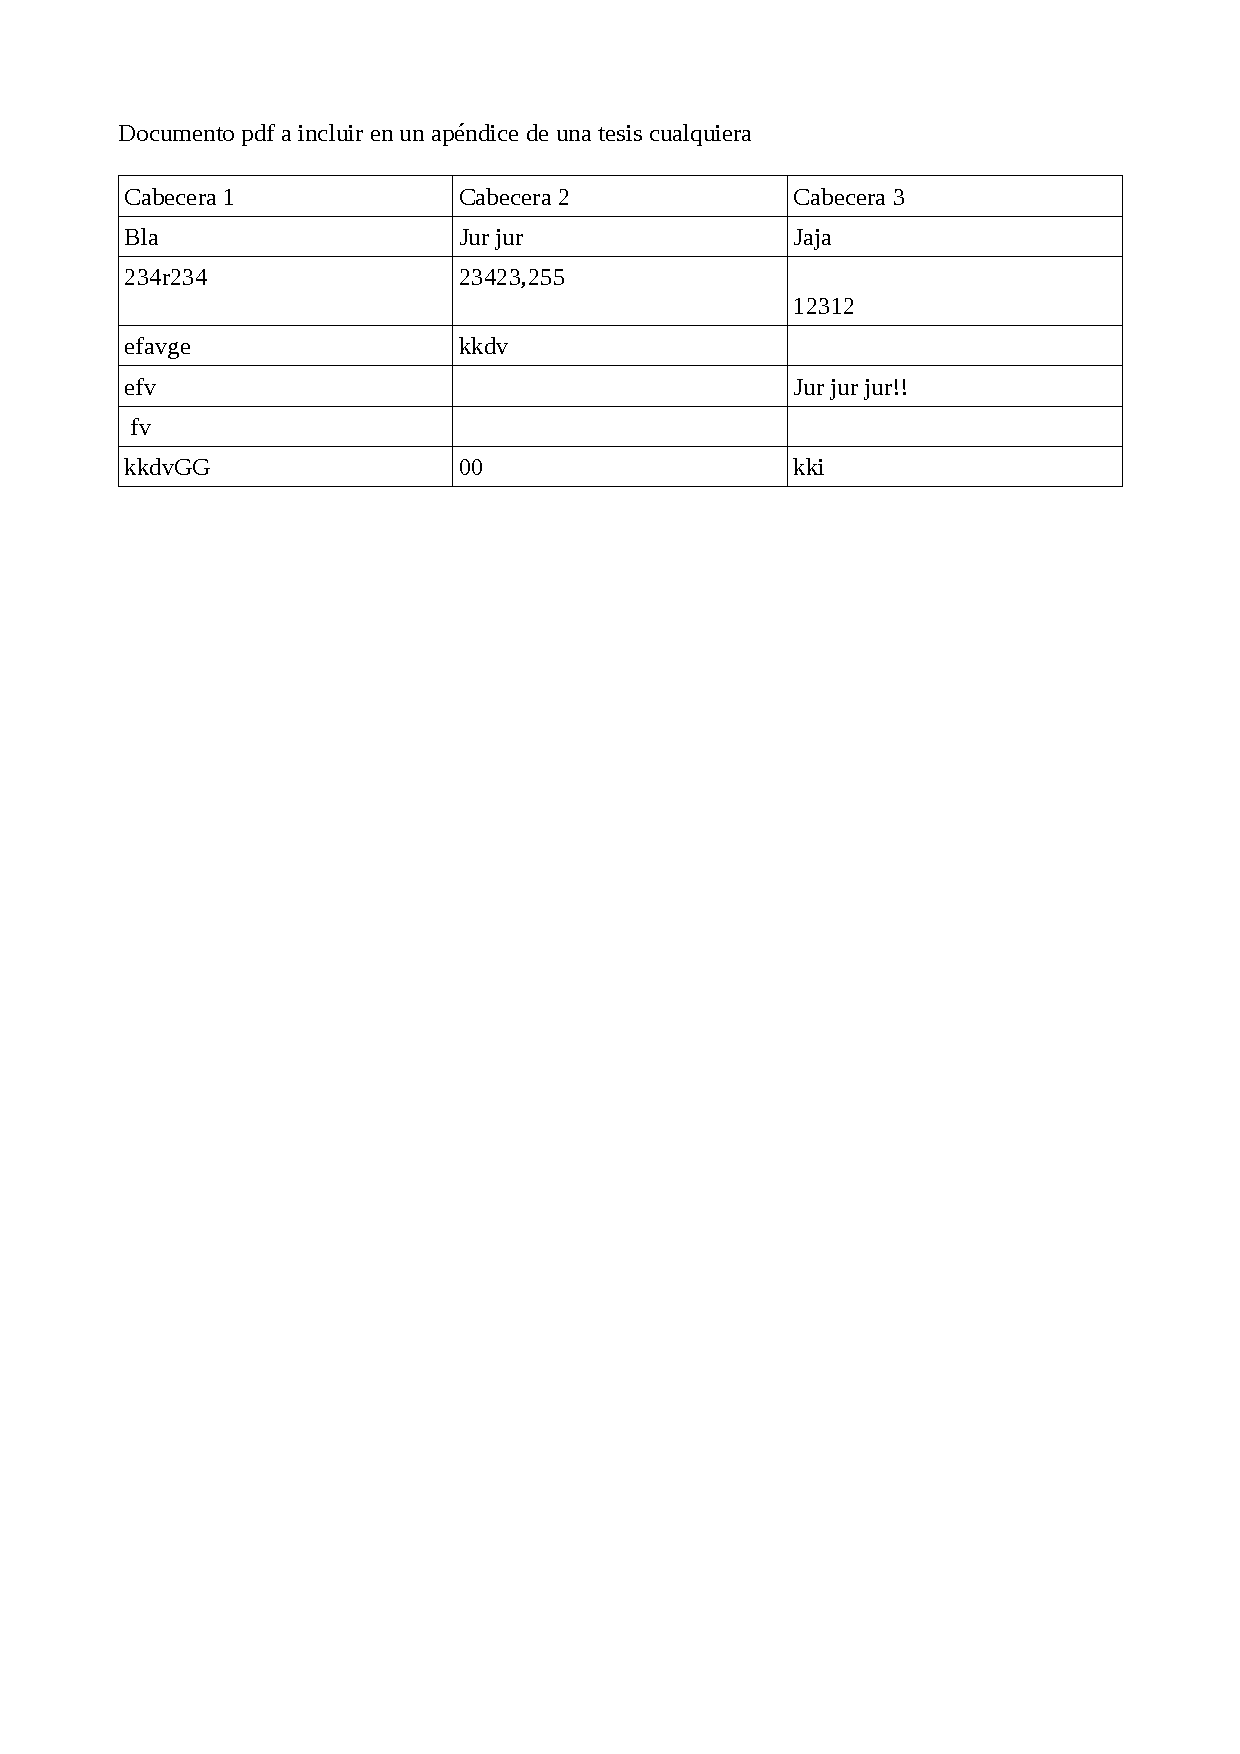
\includepdf[pages=-,templatesize={120mm}{175mm},noautoscale=false]{./elementos/otrosDocs/documento-pdf-de-ejemplo.pdf}

% \chapter{Esto será otro apéndice que es un PDF}\label{Apendice_D}
% 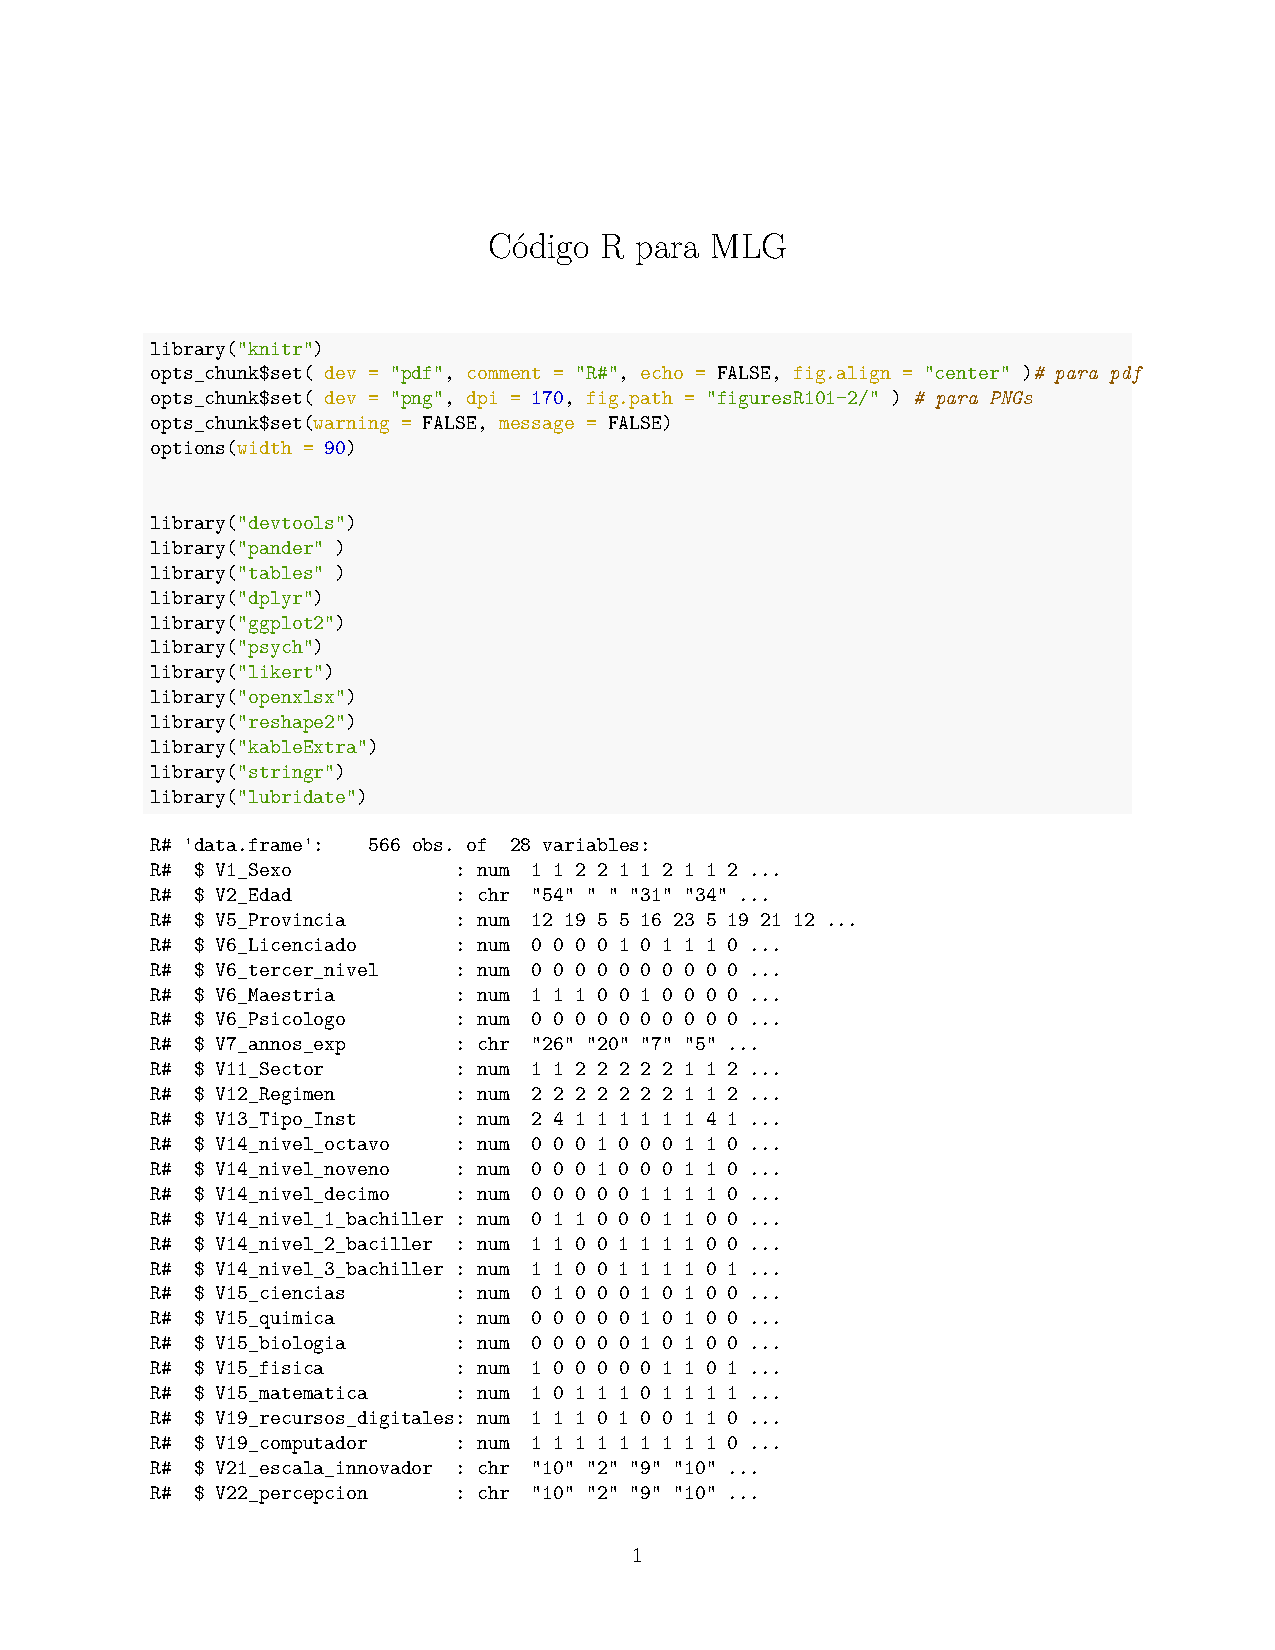
\includepdf[pages=-,templatesize={120mm}{175mm},noautoscale=false]{./elementos/otrosDocs/codigo.pdf}

\newpage %añado una página adicional blanca
\thispagestyle{empty} % empty
\mbox{}

\addtocontents{toc}{\vspace{2em}} % Agrega espacio en la toc
\end{document}









